% Created 2019-09-23 Mon 17:16
\documentclass[onecol]{ametsoc}
\usepackage[T1]{fontenc}
\usepackage[utf8]{inputenc}
\usepackage{alphabeta}
\usepackage[english]{babel}
\usepackage{array}
\usepackage{booktabs}
\usepackage{multirow}
\usepackage{longtable}
\usepackage{float}
\usepackage[normalem]{ulem}
\usepackage{etoolbox}
\usepackage{parskip}
\usepackage{paralist}
\usepackage{mathtools}
\usepackage{siunitx}
\usepackage{verbatim}
\usepackage{xfrac}
\usepackage{bigints}
\sisetup{detect-all = true, separate-uncertainty = true, list-units=single, range-units=single, range-phrase = --, per-mode=reciprocal, retain-unity-mantissa=false }
\bibpunct{(}{)}{;}{a}{}{,}
\authors{D. A. Cherian\thanks{Current affiliation: National Center for Atmospheric Research, Boulder, Colorado, USA.}\correspondingauthor{Deepak A. Cherian, NCAR, P.O. Box 3000, Boulder, CO 80307-3000.}, E. L. Shroyer}
\affiliation{College of Earth, Ocean, and Atmospheric Sciences, Oregon State University, Corvallis, Oregon, USA}
\extraauthor{H. W. Wijesekera}\extraaffil{Naval Research Laboratory, Stennis Space Center, Mississippi, USA}
\extraauthor{J. N. Moum}\extraaffil{College of Earth, Ocean, and Atmospheric Sciences, Oregon State University, Corvallis, Oregon, USA}
\journal{jpo}
\email{deepak@cherian.net}

% Here are a few math abbreviations that may be useful. Note that math
% variables should generally be set in italic, vectors in bold italic, and
% constants, such as e and i should be upright. Operators like the 'd' in
% dx  and 'D' in D/Dt should also be upright.
\newcommand{\ir}{\mathrm{i}}
\newcommand{\e}{\, \mathrm{e}} \newcommand{\er}{\mathrm{e}}

% The following makes ODEs and PDEs easier to write.
% For an example, see the second problem below. - Vallis Solution template
\newcommand{\dr}{\mathop{}\!\mathrm{d}}
\newcommand{\D}{\mathop{}\!\mathrm{D}}
\newcommand{\dd}[3][]{{\frac{\dr^{#1} #2}{\dr #3^{#1}}}}
\newcommand{\pp}[3][]{{\frac{\partial^{#1} #2}{\partial #3^{#1}}}}
\newcommand{\DD}[1]{{\frac{\D#1}{\D t}}}
% example: \pp[2]y x

\newcommand\ppx{\pp{}{x}}
\newcommand\ppy{\pp{}{y}}
\newcommand\ppt{\pp{}{t}}

% absolute value signs
% https://tex.stackexchange.com/questions/43008/absolute-value-symbols#
\DeclarePairedDelimiter\abs{\lvert}{\rvert}%
\DeclarePairedDelimiter\norm{\lVert}{\rVert}%

% Swap the definition of \abs* and \norm*, so that \abs
% and \norm resizes the size of the brackets, and the
% starred version does not.
\makeatletter
\let\oldabs\abs
\def\abs{\@ifstar{\oldabs}{\oldabs*}}
%
\let\oldnorm\norm
\def\norm{\@ifstar{\oldnorm}{\oldnorm*}}
\makeatother

% These are some of my math shortcuts
\newcommand{\mb}[1]{\boldsymbol{#1}} % math bold font
\newcommand{\ol}[1]{\overline{#1}}
\newcommand{\x}{\times}
\newcommand{\mO}{\textnormal{O}}
\newcommand{\ubr}{\underbracket}
\newcommand{\disp}{\displaystyle}
\newcommand{\vb}{\mb {v}\xspace}
\newcommand{\ub}{\mb {u}\xspace}
\mathchardef\mhyph="2D

\DeclareMathOperator{\erf}{erf}

% non-dimensional numbers
\newcommand{\Ro}{\textnormal{Ro}}
\newcommand{\Rot}{\textnormal{Ro}_\textnormal{T}}
\newcommand{\Rh}{\textnormal{Rh}}
\newcommand{\Ri}{\textnormal{Ri}}
\newcommand{\Rif}{\Ri_f}
\newcommand{\Pra}{\textnormal{Pr}}
\newcommand{\Pe}{\textnormal{Pe}}
\newcommand{\Ra}{\textnormal{Ra}}
\newcommand{\Rey}{\textnormal{Re}}
\newcommand{\Fr}{\textnormal{Fr}}
\newcommand{\Bu}{\textnormal{Bu}}

\newcommand\Hsb{H_\text{sb}}
\newcommand\tnd{t_\text{nd}}
\newcommand\bt{_\text{bot}}

\newcommand{\boxedeq}[2]{\begin{empheq}[box={\fboxsep=6pt\fbox}]{equation}{\label{#1}#2}\end{empheq}}

\newcommand{\boxedalign}[2]{\begin{empheq}[box={\fboxsep=6pt\fbox}]{align}\label{#1}#2\end{empheq}}

\usepackage{newunicodechar}
\usepackage{gensymb}
\newunicodechar{χ}{\ensuremath{\chi}}
\newunicodechar{ρ}{\ensuremath{\rho}}
\newunicodechar{ε}{\ensuremath{\epsilon}}
\newunicodechar{κ}{\ensuremath{\kappa}}
\newunicodechar{τ}{\ensuremath{\tau}}
\newunicodechar{π}{\ensuremath{\pi}}
\newunicodechar{γ}{\ensuremath{\gamma}}
\newunicodechar{ν}{\ensuremath{\nu}}
\newunicodechar{Γ}{\ensuremath{\Gamma}}
\newunicodechar{ω}{\ensuremath{\omega}}
\newunicodechar{Π}{\ensuremath{\Pi}}
\newunicodechar{°}{\degree}
\newunicodechar{≈}{\ensuremath{\approx}}
\newunicodechar{≅}{\ensuremath{\approxeq}}
\newunicodechar{≤}{\ensuremath{\le}}
\newunicodechar{≥}{\ensuremath{\ge}}
\newunicodechar{²}{\ensuremath{^2}}
\newunicodechar{³}{\ensuremath{^3}}

\setcounter{secnumdepth}{2}
\date{\today}
\title{The seasonal cycle of upper-ocean mixing at 8°N in the Bay of Bengal}
\begin{document}


\newcommand{\ML}{^\text{ML}}
\newcommand{\niw}{_\text{in}}
\newcommand{\res}{_\text{res}}
\newcommand{\niwp}{_\text{in+}}
\newcommand{\tot}{_\text{total}}
\newcommand{\low}{_\text{low}}
\newcommand{\wkb}{^\text{wkb}}
\newcommand{\Tbins}{T_\text{bins}}
\newcommand{\sort}{^\text{sort}}
\newcommand{\moor}{^\text{moor}}
\newcommand{\local}{_\text{local}}
\newcommand{\slab}{_\text{slab}}
\newcommand{\zs}{z_{*}}

% \graphicspath{images/paper1/}

\abstract{
We describe the seasonal cycle of mixing in the top \SIrange{30}{100}{m} of the Bay of Bengal as observed by moored mixing meters (χpods) deployed along 8°N between 85.5°E and 88.5°E in 2014 and 2015.
All χpod observations were combined to form seasonal-mean vertical profiles of turbulence diffusivity $K_T$ in the top 100m.
The strongest turbulence is observed between July and November during the southwest and post-monsoon seasons.
The northeast monsoon (December -- February) is a period of similarly high mean $K_T$ but an order of magnitude lower median $K_T$, a sign of energetic episodic mixing events forced by near-inertial shear events.
The months of March and April, a period of weak wind forcing and low near-inertial shear amplitude, are characterized by near-molecular values of $K_T$ in the thermocline for weeks at a time.
High mixing events coincide with the passage of surface-forced downward-propagating near-inertial waves and with the presence of enhanced low-frequency shear associated with the Summer Monsoon Current and other mesoscale features between July and October.
This seasonal cycle of mixing is consequential. 
We find that monthly-averaged turbulent transport of salt out of the salty Arabian Sea water between August and January is significant relative to local $E-P$.
The magnitude of this salt flux is approximately that required to close model-based salt budgets for the upper Bay of Bengal.
}
\maketitle

\section{Introduction}

\begin{comment}
\label{sec:org2d483eb}

\begin{itemize}
\item \textbf{reviewer 1didn't like previous introduction}. comments from reviewer 1 below:
\item "there is precious little rationale for the study provided, nor is the context of previous work much discussed in the introduction.  In fact, after a cursory first paragraph introducing the Bay of Bengal, its rivers and model predictions that vertical mixing during the Southwest monsoon is important for maintaining the Bay's salt budget, the study pretty launches into a presentation of its first results. These are the calculations of wind stress, altimetric eke,  mean surface currents, inertial energy flux and halocline dept that are intended to provide context for the study.  The problem with all of this is two-fold. Firstly, unless the authors only intend to reach readers interested in the Bay of Bengal and perhaps some upper ocean mixing people, then their introduction needs to be much broader.  Why should/would anyone else care what happens in this small region of the Indian Ocean?  Does this have a broader impact on livelihoods, ecosystems and climate change?"
\item "Secondly, in using their first results to provide context for the study, the authors commit a cardinal sin of failing to adequately describe their methods so their results can be reproduced.  The authors assume their readers are all familiar details of the datasets and non-trivial methods used - AVISO, OSCAR, MERRA-2, Alford slab-ocean mixed layer model, MIMOC etc.  These maybe widely-used datasets, but you can't assume everyone knows what they are, or what biases you may have introduced by choices in averaging, or drag coefficients. Also a few previous studies have been cited here, but as many of them would probably have done better more detailed jobs of explaining the circulation, stratification and monsoons of the Bay of Bengal, perhaps their original results should have been discussed instead of the perfunctory presentation of these we are gifted with here."
\item Objective:  This manuscript would benefit from a clear statement of the objective of the study.  Is it to provide a description of the seasonal cycle in upper ocean mixing here or address the question of whether SW monsoon-driving mixing can provide Arabian sea salt fluxes to close the  surface layer salt budgets?  Which is it? And if it is the former, then as an overarching objective, how was this justified by your rationale?
\end{itemize}

\end{comment}

The Bay of Bengal (the Bay) is the eastern semi-enclosed basin of the north Indian Ocean. 
The shallow salinity-controlled stratification in the upper Bay allows for rapid coupling with the atmosphere, and modulation of sea surface temperature (SST) within the Bay of Bengal has been linked to variations in the South Asian monsoon \citep[e.g.,][]{Vecchi2002,Roxy2014}. 
The influence of processes controlling upper ocean stratification thus extend beyond the physical footprint of the Bay. 
The Bay has a particularly strong influence on rainy and dry periods , over the Indian subcontinent, termed active and break periods respectively --- much of central India's annual rainfall results from convective systems that originate over the Bay and then propagate northwestward over the Indian subcontinent between June and September \citep{Gadgil2003a,Goswami2003}.
Interannual variations in mean rainfall are strongly correlated with fluctuations in India's agricultural output \citep{Gadgil2006}, lending significant social relevance to the problem of understanding air-sea interaction and near-surface ocean dynamics that influence the Bay's SST.

% Monsooon Intraseasonal Oscillations (MISO) are known to inter
%Building such understanding however is complicated by the immense amount of fresh water that enters the Bay every year.
%This fresh water is advected and stirred around by Ekman currents as well as the Bay's mesoscale eddy field, forming a thin \mO(\SIrange{5}{10}{m}) cap over the Bay's subsurface waters that heavily influences air-sea interaction \citep{Sengupta2016,SreeLekha2018,Rao2011}.
%This freshwater cap isolates subsurface waters from surface forcing (for example, \citealp{Lucas2016}). (\textbf{NEED BETTER CITATION FOR AIR-SEA INTERACTION}).
% Much effort has been directed recently toward understanding the fate and consequences of this fresh layer in the Bay (CITATIONS).

The Bay's physical oceanography is characterized by two major features.
First, its circulation reverses seasonally under the influence of the Indian Ocean monsoon --- the seasonal reversal of winds north of approximately 10°S in the Indian Ocean basin.
Second, it receives an immense amount of freshwater --- more than 50\% of the freshwater runoff into the entire tropical Indian ocean \citep{Sengupta2006,Gordon2016}.

The Indian Ocean monsoon and its associated precipitation is visualized in Figure \ref{fig:ppt} using seasonal mean wind stress from the Tropflux estimate \citep{Kumar2012} and precipitation from the Tropical Rainfall Measuring Mission (TRMM) Multi-satellite Precipitation Analysis dataset \citep{trmm}.
Between May and September (southwest or SW monsoon), the winds are strong and southwesterly throughout the Indian Ocean basin.
Precipitation over the Indian subcontinent is substantial (Figure \ref{fig:ppt}c).
The months of October and November (post-monsoon period, SWNE) are characterized by weak mean wind stress over most of the basin including the Bay (Figure \ref{fig:ppt}d). 
The seasonal averaging hides the episodic presence of strong cyclones in the Bay that bring large amounts of rain and significantly affect lives of those residing along the perimeter of the Bay.
Recent examples of cyclones that strengthened over the Bay and made landfall resulting in loss of life and severe damages, include Category 5 Tropical Cyclone Phailin in October 2013 and Category 4 Tropical Cyclone Hudhud in October 2014.
% Sri Lanka in particular receives a substantial fraction of its annual mean precipitation during this season.
The mean winds strengthen in December and switch to being northeasterly up until February (northeast or NE monsoon).
These winds are weaker than those during the SW monsoon.
Nations on the Bay's Rim i.e. India and Sri Lanka receive relatively little rainfall during this period and the precipitation maximum is located over the Bay (Figure \ref{fig:ppt}a).
The months of March and April are a period of weak winds and almost no precipitation north of 4°N (northeast-southwest transition, NESW; Figure \ref{fig:ppt}b).

The monsoon cycle of wind forcing described above imprints seasonality on the Bay's circulation (\citealp{Schott2002,Shankar2002}).
The East India Coastal Current (EICC) spins up at the Bay's western boundary during both monsoons, flowing northward between May and October and then southward between December and April.
The EICC is readily visible in seasonally-averaged estimates of near-surface ocean velocity (vectors in Figure \ref{fig:spatial}a--e from the Ocean Surface Current Analysis Real-time product, OSCAR; \citealp{Bonjean2002}).
(OSCAR is a diagnostic estimate at five-day frequency that ignores local acceleration and nonlinearities but accounts for geostrophic, thermal wind and Ekman currents.)
The EICC exists as a discontinuous flow with many recirculation loops and is visible as a local maximum along India's eastern coast in maps of geostrophic eddy kinetic energy \(\text{EKE} = 0.5[u_g^2 + v_g^2]\) (colored field in Figure \ref{fig:spatial}a--e; \citealp{Durand2009}).
Here \((u_g, v_g)\) are geostrophic velocity anomalies computed from delayed-time sea surface height estimates as measured by multiple satellite altimeters by the Copernicus Marine Environment Monitoring Service (CMEMS)\footnote{DT all-sat-merged Global Ocean Gridded SSALTO/DUACS Sea Surface Height L4 product and derived variables (dataset-duacs-rep-global-merged-allsat-phy-l4-v3).}. 
Apart from the EICC, one other major circulation feature is the Summer or Southwest Monsoon Current (SMC).
The SMC is visible in the seasonal mean during the SW monsoon as an eastward jet along 8°N between 85°E and 92°E in Figure \ref{fig:spatial}d (vectors).
Peak velocity in the SMC can exceed \SI{1.5}{\meter\per\second} and northward transport has been estimated to be in the range \SIrange{10}{27}{Sv} though some of this transport may be due to recirculations \citep{Wijesekera2016a,Vinayachandran1999,Webber2018}.
The southwestern and south-central Bay is a site of energetic mesoscale variability during the SW monsoon (our Figure \ref{fig:spatial}d; \citealp{Chen2018}).
The elevated EKE reflects at least three mesoscale features: a westward propagating anticyclone \citep{Wijesekera2016a}, a large cyclonic eddy that spins up annually off the coast of Sri Lanka (the Sri Lanka Dome, \citealp{Vinayachandran1998}) and the SMC which threads a pathway between the Sri Lanka Dome to the north and the anticyclone to the south \citep{Vinayachandran1999,Wijesekera2016a}.
During the NE monsoon, the mean circulation in southern Bay reverses and the Northeast Monsoon Current (NMC) flows westward with a weaker signal in EKE (Figure \ref{fig:spatial}a,b).

Large outflows from the Ganga, Brahmaputra, and Irrawady rivers, and substantial precipitation make the Bay a strongly salinity-stratified basin in its near-surface depths particularly toward the north. The annual river discharge peaks towards the end of the SW monsoon and the fresh water is eventually exported out along the Bay's western and eastern margins \citep{Sengupta2006}. The exported water is saline with \(S \approx 34 \mhyph 35\) \si{psu}. Hence maintaining the Bay's long term salt balance requires both an inflow of salty water from outside the Bay and the upward turbulent transport of that imported salt so as to permanently modify the near-surface freshwater \citep{Vinayachandran2013}.

The western half of the north Indian Ocean, the Arabian Sea, is generally considered the source of the required salty water \citep[for example, ][]{Jensen2001}, although recently \cite{Sanchez-Franks2019} used a multiyear model to argue that the original source of the salty water is the western equatorial Indian Ocean. Regardless of specific source, both observations and models agree that the SMC is the dominant pathway for salty water entering the Bay \citep{Jensen2001,Vinayachandran2013,Webber2018}\footnote{Recent observations and model simulations describe a second pathway — a persistent subsurface inflow of salty water during the NE monsoon that exists as a superposition of frequent salty intrusion events that average out to a region of broad northward flow of high salinity water west of 85°E \citep{Wijesekera2015,Jensen2016}.}.
The salty signature of the SMC is visible in maps of the depth of the 34.75 isohaline surface which shallows by \SI{25}{m} or so in the southwestern Bay during the summer monsoon (Figure \ref{fig:spatial}k--o; \citealp{Murty1992a,Vinayachandran2013}).
The shallow depth of the \(S = \SI{35}{psu}\) isohaline in the southwestern and south-central Bay relative to the northern Bay led \cite{Vinayachandran2013} to hypothesize that the southern Bay is a site of enhanced mixing and associated salt fluxes that may be an important contributor to the salt budget of the Bay.
In agreement with this hypothesis, model studies have implicated vertical mixing as the primary mechanism for diluting the immense amount of fresh water the Bay receives during the southwest monsoon \citep{Akhil2014,Benshila2014,Wilson2016a}.

%\begin{itemize}
%\item \textbf{need a little help finishing the introduction}
% \item \textbf{also, given the reviewer comments, I removed all discussion of Figure 1f-j. Those panels are only discussed in the results section. Is that OK?}
%\end{itemize}

Here, we summarize year-long direct observations of turbulence at three moorings along 8°N in the south-central Bay (white dots in Figures \ref{fig:ppt}, \ref{fig:spatial}). We show that the seasonal cycle of winds and currents described above is imprinted on mixing in the Bay with near-molecular mixing during the quiet transition period giving way to elevated mixing during both monsoon periods primarily associated with near-inertial shear (Sections \ref{sec:results}\ref{sec:profile}, \ref{sec:discussion}\ref{sec:seasonal}). The observed seasonal cycle in mixing is likely significant for the Bay's salt budget as has been previously hypothesized (Section \ref{sec:discussion}\ref{sec:js}). We find that the upward turbulent salt transport out of subsurface high salinity water at 8°N is comparable to freshwater gained through precipitation (less evaporation).


\section{Observations}
\label{sec:org8690ffb}
\label{sec:obs}

\subsection{χpod}
\label{sec:org94fefd7}
\label{sec:pod}

All presented turbulence quantities were obtained using χpods: self-contained instruments each consisting of two fast-response FP-07 thermistors, a pitot-static tube for high-frequency speed measurements, a pressure sensor, a compass, and accelerometers \citep{Moum2009a,Moum2015}.
Refinement over many years has resulted in a system that can return records of turbulent temperature fluctuations for up to a year or more.
The two thermistors on the χpod record temperature fluctuations at 100Hz.
Temperature gradient spectra are computed using 1 second data intervals and are fit to the theoretical spectrum of \cite{Kraichnan1968} in the viscous-convective range \citep{Moum2009a}.
The Kraichnan spectrum is a function of two quantities: the turbulence dissipation rate of temperature variance \(χ\) and the turbulence dissipation rate of kinetic energy \(ε\), but the χpods only record one quantity, temperature.
The dependence on \(ε\) arises from the \cite{Batchelor1959} wavenumber which marks the end of the viscous-convective range.
Since χpod thermistors do not resolve the Batchelor wavenumber typically (e.g. \citealp{Lueck1977}), fitting the Kraichnan spectrum requires specification of \(ε\).
In the absence of an independent estimate of \(ε\), we assume that the turbulence diffusivities of temperature  \(K^t_T = χ/2/T_z^2\) and density \(K^t_ρ = Γε/N^2\) are equal with mixing efficiency \(Γ = 0.2\) for stratified turbulence (\citealp{Osborn1972}; \citealp{Osborn1980}; and \citealp{Gregg2018} respectively).
This yields a relationship between \(χ\) and \(ε\), 
\begin{equation}
    \label{eq:eps}
    ε = \frac{N² χ}{2 Γ T_z²}
\end{equation}
and a solution is obtained by fitting the spectrum through the iterative procedure described in \cite{Moum2009a}.
The buoyancy frequency \(N\) and vertical temperature gradient \(T_z\) are estimated using two CTD instruments deployed above and below the χpod.
\emph{In-situ} comparisons between χpod estimates and more ``standard'' estimates from vertical microstructure profiles are favorable under stably-stratified sheared conditions \citep{Perlin2012,Pujiana2018}.
Total temperature and salt diffusivities \(K_T, K_S\), heat flux \(J_q^t\) and salt flux \(J_s^t\) are estimated from a time series of \(χ\) using
\begin{subequations}
\label{eq:def}
 \begin{align}
  K_T &= κ_T(S,T,P) + \frac{χ/2}{T_z^2}, \\
  K_s &= κ_s + \frac{χ/2}{T_z^2}, \\
  J_q^t &= - ρ_0\, c_p\, K_T\, T_z, \\
  J_s^t &= - ρ_0 \, K_S \, S_z;
\end{align}
\end{subequations}
where \(κ_T, κ_s\) are the molecular diffusivity of temperature and salinity respectively, and \(T_z, S_z\) are background temperature and salinity gradients (usually obtained by differencing nearby CTDs on the moorings; subscript \(z\) indicates \(z\)-derivative).
Again we have assumed that high Reynolds number geophysical turbulence mixes all scalars at the same rate so that the \emph{turbulence} diffusivities of both temperature and salinity are equal i.e. \((χ/2)/T_z^2\).

A challenge with analyzing χpods deployed in the Bay's thermocline is the frequent occurrence of weakly turbulent and near-laminar flow for extended periods of time as has been recorded with microstructure measurements in the Aegean Sea \citep{Gregg2012} and in the Arctic \citep{Scheifele2018}.
Analyzing microstructure measurements in such environments is challenging given that the usual assumptions of isotropy, steadiness and homogeneity break down \citep{Rohr1988,Itsweire1993,Gargett1984a}.
The χpod records ``bit noise'' when the turbulent temperature fluctuations are below the FP-07 sensor's detection threshold.
We can account for such behaviour using knowledge of the  circuit components involved (Appendix B).
When the recorded temperature variance of an one second subset of data is within an arbitrary factor of 1.5 of the inferred noise variance of the sensor, we set \(ε\) to NaN and \(χ\) to 0 resulting in \(K_T, K_S\)  being set to molecular values \(κ_T, κ_S\) and the resulting fluxes \(J_q^t, J_s^t\) being that due to molecular diffusion (eqn. \ref{eq:def}).
We do so following \cite{Gregg2012} with the understanding that setting \(χ\) to any non-zero value during such periods seems unjustifiable.


\subsection{The 2014-2015 Bay of Bengal deployment}
\label{sec:org46e574a}

As part of the U.S. Office of Naval Research's Air Sea Interaction Regional Initiative (ASIRI) and the Naval Research Laboratory's (NRL) Effects of Bay of Bengal Freshwater Flux on Indian Ocean Monsoon (EBoB) programmes a number of moored mixing meters  \citep[χpods,][]{Moum2009a} were deployed on moorings in the southwestern Bay.
This paper focuses on three moorings deployed along 8°N east of Sri Lanka in late December 2013 (Figure \ref{fig:map}a and Table \ref{tab:pods}).
The χpods ended up at a variety of depths and returned data up to February 2015 (Table \ref{tab:pods}, Figure \ref{fig:map}b--i and \citealp{Wijesekera2016a}).
Nearly all were predominantly in the main thermocline (Figure \ref{fig:map}b--e) and sampled the high salinity water associated with the Summer Monsoon Current (SMC) during the summer monsoon (Figure \ref{fig:map}f--i).
This region experiences a significant seasonal cycle in near-surface velocity and mesoscale eddy kinetic energy (Figure \ref{fig:spatial}a--e).
The moorings were displaced by up to 50m (``blowdown'') by mesoscale features when present.

Two Teledyne RD Instruments ADCPs were deployed at the top of each mooring: an upward-looking Workhorse \SI{300}{kHz} sampling every half hour in \SI{2}{m} bins and a downward-looking Long Ranger \SI{75}{kHz} sampling every hour in \SI{8}{m} bins (further details are available in \citealp{Wijesekera2016a}).
A data gap in velocity coverage exists between the two ADCPs that is approximately \SI{21}{m} wide.
The shallower χpod was deployed within the blanking zone of the downward looking ADCP, so shear can be directly estimated only at the deeper χpod.
We estimate shear by first interpolating the velocities over the gap in depth, central differencing the interpolated velocity over three \SI{8}{m} wide bins, and then reintroducing the gap.
Each mooring contained more than fifteen temperature sensors of various kinds distributed between the buoy and \SI{352}{m} below the buoy.
Salinity coverage was coarser with four sensors deployed within a \SI{50}{m} depth below the buoy and one sensor at \SI{352}{m} \citep{Wijesekera2016a}.
Three of the four shallow salinity sensors were concentrated around the two χpods deployed \SI{12}{m} and \SI{32}{m} below the buoy.

\section{Results}
\label{sec:results}

Much of this manuscript describes a seasonal cycle in thermocline turbulence that coincides with a seasonal cycle in thermocline shear.
The seasonal variation in turbulence will be discussed along with the seasonal variation in the shear field, decomposed into three components as described below.
Bursts in near-inertial shear will be linked back to surface winds using an approximate estimate of mixed-layer wind energy input obtained using a slab mixed layer model, also described below.
First we introduce and rationalize our decomposition of the shear field.
%Then we describe our construction of a seasonally averaged vertical profile (Section \ref{sec:results}\ref{sec:profile}).
%Later in Section \ref{sec:results}\ref{sec:nrl}, we present time series of turbulence and shear at a single χpod and discuss the seasonal cycle implied by each of these figures in more detail (Section \ref{sec:results}\ref{sec:seasonal}).

\subsection{Seasonal cycle in observed vertical shear}
\label{sec:shear}

At all three moorings, \emph{Eulerian} rotary spectra of vertical shear \(S\tot = \sqrt{u_z^2 + v_z^2}\) at \SI{152}{m} depth\footnote{We choose \SI{152}{m} to avoid any uncertainties with having to interpolate over the gap in ADCP coverage} are dominated by a broad peak at \(-f_0\) (40\%--60\% of sampled variance), narrow secondary peaks at \(-f_0 \pm ω_{M2}\) (\(ω_{M2}\) is the \(M_2\) tidal frequency, 5\%--10\% variance) and distributed variance at frequencies less than \SI{10}{days} reflecting meanders of the Summer Monsoon Current (20\% variance).
These spectra are presented in Figure \ref{fig:nrlspectra}a,c,e (clockwise in black, counterclockwise in red).
The narrow peaks at \(-f_0 \pm ω_{M2}\) are a sign of vertical advection or pumping of near-inertial shear layers by the \(M_2\) tide which Doppler-shifts spectral energy from \(-f_0\) to \(-f_0 \pm ω_{M2}\) \citep{Alford2001a}.
The effect of tidal pumping can be removed by estimating the spectra in isopycnal space (e.g. \citealp{Alford2017}).
Given the sparse sampling in salinity, we instead estimate spectra in \emph{isothermal} space.
The peaks at \(f_0 \pm ω_{M2}\) are much less prominent at the $T=\SI{18}{\celsius}$ isotherm at all moorings (annual mean depth 150m; Figure \ref{fig:nrlspectra}b,d,f), leading us to interpret the near-tidal peaks in the Eulerian spectra (Figure \ref{fig:nrlspectra}a,c,e) as primarily being near-inertial shear that is Doppler shifted to near-tidal frequencies.
Ideally we would interpret the χpod mixing estimates using a time series of isothermal shear that is filtered to isolate the low frequency and near-inertial components.
It is not possible to obtain a gapless estimate of these filtered components given the gap in ADCP coverage.
Instead we proceed by conducting our analysis in the Eulerian frame as follows.

We decompose the total vertical shear \(S\tot\) by linearly interpolating over the sampling gap in the vertical and then using a second-order Butterworth filter applied forwards and backwards to split the shear time series into four components: (a) low-frequency shear \(S\low\) (lowpass with half power point 9 days), (b) near-inertial shear  \(S\niw\) (bandpass between half power points 7 days and 2 days respectively), (c) near-tidal shear (bandpass between half power points 15.3 hours and 10.4 hours\footnote{0.95(\(ω_{M2} - f_0\)) to 1.05(\(ω_{M2} + f_0\))}) and (d) a residual \(S\res\).
These frequency ranges are shaded in Figure \ref{fig:nrlspectra}.
Given the previous discussion, we incorporate near tidal shear with \(S\niw\).
The combined sum \(S\niwp\) represents any shear associated with near-inertial waves, advection of near-inertial waves by the tide as well as any tidal shear.

Depth-time maps of the mean squared shear for three shear components \(S\low, S\niwp, S\res\) along with the total shear \(S\tot\) are shown in Figure \ref{fig:shears}.
At all three moorings, energetic shear is observed in January, February, and for an extended period between July and November.
The shear field is relatively weak between mid-March and the beginning of June.
Episodic energetic bursts in near-inertial shear are seen at all three moorings outside these months.
All three moorings see a large rise in low-frequency shear between July and November.
This is an indication of the Sri Lanka Dome and a large anticyclonic eddy through the array as the meandering of the Summer Monsoon Current (note EKE maximum inferred from altimetric data in Figure \ref{fig:spatial}a--e).
The magnitude of the low-frequency shear is comparable to that of near-inertial shear at all three locations during the SW monsoon.
% At NRL4, the low-frequency, near-inertial and residual components contribute equally to total shear.
The residual \(S\res\) is generally weak relative to the \(S\low\) and \(S\niwp\).
The episodic nature of near-inertial shear events prevent a confident estimation of the magnitude of its seasonal cycle given that only one annual cycle is resolved.
However the seasonal signal in \emph{total} shear — high shear between June and February, and low shear between March and June — is robust and consistent across all three moorings.


\subsection{Seasonal cycle in near-inertial energy input}
\label{sec:org2f661af}
\label{sec:input}

We provide context for the observed near-inertial shear events by using a slab mixed layer model to estimate wind-forced energy input \(Π\) in to the mixed layer. % Previous work has linked shear associated with wind-forced downward-propagating near-inertial waves to thermocline turbulence \citep{Alford2001b,Whalen2018}.
 We follow \cite{Alford2003} and obtain a slab model estimate of \(Π\), \(Π\slab\), by forcing a slab ocean mixed layer model with reanalysis 10-m winds at hourly frequency (MERRA-2, the Modern-Era Retrospective Analysis for Research and Applications, Version 2, \citealp{Gelaro2017}) and using climatological monthly mixed layer depths from the Monthly Isopycnal Upper-Ocean Climatology with Mixed Layers dataset (MIMOC, \citealp{Schmidtko2013}).
Details of the solution are described in Appendix A.

The SW monsoon winds drive moderate near-inertial flux nearly uniform throughout the Bay (Figure \ref{fig:spatial}f--j).
The largest near-inertial fluxes over the year are confined to latitudes south of 10N until the months of October and November when strong input associated with the passage of Tropical Cyclone Hudhud (October 5-14, 2014) occurs between 12°N and 16°N.
Intense near-inertial input in the Bay is forced by the passage of cyclonic systems as in the mid-latitudes \citep{Alford2003} --- the tracks of Very Severe Cyclonic Storm Madi (December 7-11, 2013) and Depression BOB01 (January 2-6, 2014) are readily visible in the near-inertial input field for the NE monsoon.
There is little to no near-inertial energy flux into the mixed layer during March (northern Bay) and April (entire Bay).


\subsection{Seasonal cycle in mixing}

We illustrate the seasonal cycle of turbulence in two ways:
 (a) by first presenting a time series of daily-averaged observations at a single mooring (NRL5, Figure \ref{fig:nrl}), and
 (b) by presenting a seasonally averaged vertical profile of diffusivity that synthesizes observations from all three moorings (Figure \ref{fig:vert}).

\label{sec:orgbcce381}
\subsubsection*{A prototypical time series (NRL5; 8°N, 88.5°E)}
\label{sec:org1c0c44b}
\label{sec:nrl}

We present the seasonal cycle of winds, turbulence, shear and stratification at mooring NRL5 using daily averaged quantities in Figure \ref{fig:nrl}.
We choose to highlight mooring NRL5 for two reasons.
First, it experiences the least blowdown and is least contaminated by the associated space-time aliasing (\SIrange{10}{20}{\meter}, Figure \ref{fig:nrl}f).
Second, the turbulence quantities in Figure \ref{fig:nrl} are inferred from measurements recorded by the deep χpod at 105m.
This instrument is the deepest deployed in the Bay to date, and recorded the longest period of weak turbulence observed during the transition months of March and April.
The filtered shear components shown in Figure \ref{fig:nrl}d are obtained by first subsampling the filtered depth-time fields along the χpods trajectory and then normalizing by 30-day lowpass filtered \(N²\).
Time series recorded at the other moorings are presented in the Supplementary Material.

Mixing events during the NE monsoon are episodic and relatively weak ($K_T \le \SI{1e-6}{\metre\squared\per\second}$) while the transition months of March and April are a period of extremely weak mixing.
The χpod measures sustained and relatively high mixing between the months of May and October --- a period of energetic mesoscale activity and moderately large near-inertial energy input \(Π\) in the south-central Bay (Figures \ref{fig:spatial}).
The Summer Monsoon Current arrived at NRL5 in July, bringing in high salinity water and reducing \(N^2\) (Figure \ref{fig:nrl}d).
Its arrival coincided with the rise of \(K_T\) to sustained values greater than \SI{1e-6}{\meter\squared\per\second}.
However \(K_T\) was still consistently below and rarely exceeded the canonical mid-latitude thermocline value of \SI{1e-5}{\m\squared\per\s} (\(50κ_T\), Figure \ref{fig:nrl}b).
Heat flux \(J_q^t\) is likewise small and exceeds \SI{10}{\W\per\m\squared} for only a few days in the entire year (Figure \ref{fig:nrl}c).

\subsubsection*{A seasonally varying vertical profile of diffusivity \(K_T\)}
\label{sec:org56f20f8}
\label{sec:profile}

We synthesize all χpod observations along 8°N by constructing approximate seasonally-averaged vertical profiles of \(K_T\), presented in Figure \ref{fig:vert}, as follows:
\begin{enumerate}
\item We label every averaged \(K_T\) measurement with the density value of the parcel as well as the depth of measurement.
\item All measurements are then binned by density with bin edges [1018, 1021, 1022, 1022.5, 1023, 1023.5, 1024.25, 1029] \SI{}{\kg\per\m\cubed}.
\item For each season, we construct a PDF of \(K_T\) in each bin and calculate the mean and standard deviation of the depths of measurement.
\item The PDFs are presented at the mean depth of the density bin as a vertical profile (Figure \ref{fig:vert}). Each PDF is labelled with the mean density in each bin; means and medians are marked by circles and diamonds respectively (see caption).
\end{enumerate}
% The moorings are blown down by as much as \SIrange{50}{70}{m} by the Summer Monsoon Current between July and September.
Some considerations must be kept in mind while interpreting Figure \ref{fig:vert}.
First, our definition of seasons need not line up perfectly with periods of relatively high or relatively low winds or mixing at every mooring.
Second, the χpods on the NRL3 mooring appear to be within the mixed layer and the isothermal but salinity-stratified barrier layer for a few weeks in February.
These measurements are excluded since we do not have enough observations to construct meaningful averages for the mixed and barrier layers.
Third, Figure \ref{fig:vert} ignores all spatial variability.

Despite these caveats, Figure \ref{fig:vert} presents a useful summary of observed mixing along 8°N.
There is a clear seasonal cycle in turbulent diffusivity in the upper 30--100m at the mooring locations just as at NRL5 (Figure \ref{fig:nrl}).
Vertical profiles of both mean and median values of \(K_T\) are always surface intensified (tables of both means and medians are provided in Appendix B).
The amplitude of the seasonal cycle in mean diffusivities is roughly an order of magnitude with mean $K_T \approx \SI{1e-4}{\metre\squared\per\second}$ during both monsoons.
Median $K_T$ is approximately an order of magnitude larger during the SW monsoon as compared to the NE monsoon (\SI{1e-6}{\metre\squared\per\second} versus \SI{1e-7}{\metre\squared\per\second}) indicating that energetic mixing events are rarer during the NE monsoon.
The most striking feature of Figure \ref{fig:vert} is the near-complete lack of mixing in the south-central Bay's thermocline during the months of March and April --- median diffusivity values are only slightly greater than molecular diffusivity \(κ_T\) at depths greater than \SI{60}{m}.
The observation of near-molecular diffusivity at the deep χpod at NRL5 is thus consistent across the other two moorings.

\section{Discussion}
\label{sec:discussion}
\label{sec:org615d810}
\subsection{A seasonal cycle in shear and turbulence}
\label{sec:orgbe17f73}
\label{sec:seasonal}

We now describe the seasonal cycle of shear and turbulence by synthesizing Figures \ref{fig:shears}, \ref{fig:nrl} and \ref{fig:vert}.


\subsubsection*{NE monsoon (December -- February)}
\label{sec:org19b69a2}

During the NE monsoon, mean \(K_T ≥ \SI{1e-5}{\m\squared\per\s} (50κ_T)\) and medians are lower by one to two orders of magnitude across all three morings (Figure \ref{fig:vert}).
All three ADCPs recorded the passage of energetic packets of near-inertial energy in January and February (Figure \ref{fig:shears} and \ref{fig:nrl}e).
These packets are likely associated with the passage of Cyclonic Storm Madi and Depression BOB01, whose tracks are visible in the near-inertial input \(Π\slab\) (Figure \ref{fig:spatial}f).
Between December and February, the deep χpod at NRL5 records relatively weak turbulence with maximum \(K_T \approx \SI{1e-6}{\meter\squared\per\second}\).
Note that the near-inertial event is weakest at NRL5, Figure \ref{fig:shears}i.

\subsubsection*{Transition (March -- April)}
\label{sec:org10f739a}

Arguably, the most dramatic observation is that the χpod at 105-m recorded near-laminar flow in the thermocline i.e. near-molecular values of \(K_T\) during the \emph{entire} month of April.
Similar periods of low to negligible mixing are present at other χpods, but for shorter periods of time.
Median \(K_T ≤ \SI{1e-6}{\m\squared\per\s} \approxeq 5κ_T\) in most thermocline density bins (deeper distributions in Figure \ref{fig:vert}), i.e. the observation of weak to negligible mixing is consistent across all locations.
The transition months of March and April are a period of weak thermocline currents, weak thermocline shear, weak winds, high net surface heat flux and low near-inertial energy flux (Figures \ref{fig:spatial}, \ref{fig:shears} and \ref{fig:nrl}). These conditions are consistent with the observations of weak mixing.
Weak pulses of near-inertial shear are seen in Figures \ref{fig:shears} and \ref{fig:nrl}e; again this is consistent with weak wind forcing at the surface (Figure \ref{fig:spatial}k--o).
Stratification is relatively high at all χpod depths: $N² \sim \SI{5e-4}{\per\second\squared}$.

\subsubsection*{SW monsoon (May -- September)}
\label{sec:orgec06087}

With the onset of the SW monsoon, the χpods observe an order of magnitude increase in mean \emph{thermocline} diffusivity to \(K_T \approx \SI{1e-4}{\m\squared\per\s} (500κ_T)\) with peak values of \(K_T \approx \SI{1e-2}{\m\squared\per\s} (\num{5e4}κ_T)\) between July and September (Figure \ref{fig:vert}).
The mean diffusivity is two to four orders of magnitude larger than values observed during March and April (Figure \ref{fig:vert}).
Median thermocline diffusivities during the SW monsoon are larger relative to the NE monsoon by a factor of 5 -- 10 (Figure \ref{fig:vert} and Table B2).
The medians are also closer to the means during the SW monsoon (Figure \ref{fig:vert}), as compared to the NE monsoon, an indication of persistent mixing events.

The SMC and other mesoscale features are visible in \(S\low\) at all three moorings during this season though for differing lengths of time (Figure \ref{fig:shears}).
Both seasonal mean surface velocities from the OSCAR product and mooring ADCP data show the mesoscale to be prominent especially at NRL3 and NRL4, the two westernmost moorings along 8°N (also see Figures \ref{fig:spatial}a--e, \ref{fig:hov} and \citealp{Wijesekera2016a}).
This inference is consistent with the ADCP measurements (Figure \ref{fig:shears}). At NRL5, elevated mixing occasionally lines up with short periods of elevated low frequency shear between May and October (Figure \ref{fig:nrl}e).

A few high mixing events are also associated with bursts of elevated near-inertial shear that last for one to two weeks at a time at NRL5 (Figure \ref{fig:nrl}e).
The maximum observed diffusivity and turbulence fluxes in Figure \ref{fig:nrl} coincide with the passage of a particularly strong set of near-inertial wave packets that forced enhanced turbulence at the χpod's depth (July 25 -- August 7, highlighted in white in Figure \ref{fig:nrl}b,c).
Zonal shear and \(K_T\) for this period of intense mixing are shown in Figure \ref{fig:nrl5-niw}.
The elevated mixing coincides with the passage of a set of \(M_2\) tide packets that vertically displace the isotherms and the near-inertial shear in Figure \ref{fig:nrl5-niw}b.
The effect of tidal vertical advection can be removed by interpolating to isothermal or isopycnal space \citep{Alford2001a}.
In doing so, we see that squared near-inertial shear is larger than near-tidal shear on both isotherms by nearly an order of magnitude (Figure \ref{fig:nrl5-niw}c).
It is such vertical advection that results in Doppler shifted spectral peaks at \(-f_0 \pm ω_{M2}\) (Figure \ref{fig:nrlspectra}).
Hence we interpret the apparent modulation of \(K_T\) at near-\(M_2\) frequency (Figure \ref{fig:nrl5-niw}a) as a result of the \(M_2\) tide heaving near-inertial shear layers past the χpod, and not mixing forced by tidal shear.


\subsubsection*{Post-monsoon (October -- November)}
\label{sec:orgdf40b13}

Energetic turbulence is observed at the NRL3 and NRL4 moorings during October and November (see \(ρ-1000 = 22.2,\  22.8\) and \SI{23.2}{\kg\per\m\cubed} bins in Figure \ref{fig:vert}).
Surface velocities in the OSCAR dataset suggest that the SMC ceases to exist as a continuous inflow through the Bay's southern boundary at the end of September.
Subsequent periods of enhanced low frequency shear in Figure \ref{fig:nrl}e between October and January appear to be associated with westward propagating features seen in OSCAR surface velocity data (Figure \ref{fig:hov}).
At NRL3, energetic mixing is recorded by the shallower χpod during October; unfortunately the gap in ADCP coverage prevents us from attributing this turbulence to a specific shear event.
At NRL4 the χpods record high mixing during November; again this coincides with a downward propagating near-inertial wave (Figure \ref{fig:shears}h).
There are two strong wind events at the surface in October and November (Figure \ref{fig:nrl}a) that are likely responsible for downward propagating near-inertial energy during this season (Figures \ref{fig:shears}; also see enhanced \(Π\slab\) in Figure \ref{fig:spatial}f--j).
At NRL5, there appears to be some mixing associated with a low-frequency shear peak in October (Figure \ref{fig:nrl}b,e).

Despite the above noted tendency, near-inertial shear did not always correspond with high mixing. For example, negligible mixing is associated with a burst in near-inertial shear in November (Figure \ref{fig:nrl}b,e). This wave packet appears to have forced turbulence at a depth not sampled by the χpods, if at all. Enhanced near-inertial shear need not necessarily lead to mixing. \cite{Alford2001b} observe that peak mixing associated with a downward propagating near-inertial wave occurs at the stratification maximum. As they point out, this is consistent with WKB scaling: the Froude number scales with stratification \(\Fr = S/N \sim N^{1/4}\) so shear instability is expected at the stratification maximum. A χpod would need to be at the right depth relative to the stratification structure to observe turbulence forced by near-inertial energy --- a major caveat to our analysis.


\subsubsection*{Summary}
\label{sec:org78d8996}

There is a strong seasonal cycle in thermocline mixing (Figure \ref{fig:vert}) that appears to be linked to a seasonal cycle in thermocline shear (Figure \ref{fig:shears}).
The seasonal cycle in shear results from
(a) the seasonal presence of the Summer Monsoon Current which greatly increases low-frequency shear \(S\low\) between July and October, and
(b) episodic energetic downward propagating near-inertial waves observed outside March and April.
At times, \(S\low\) is of comparable magnitude to near-inertial shear \(S\niwp\) (Figure \ref{fig:shears}).
The seasonal cycle in low-frequency shear is expected from the well established seasonal spinup and spindown of the SMC and the Sri Lanka Dome \citep{Schott2001a, Vinayachandran1998}.
A seasonal cycle in near-inertial shear is perhaps expected from the seasonal cycle of winds.
However our ADCP record cannot sufficiently characterize the magnitude of the seasonal cycle in near-inertial energy, given the small number of large magnitude near-inertial events at all three moorings (Figure \ref{fig:shears}).
% Next we examine the consequences of turbulent mixing in the thermocline.

\subsection{Weak turbulence in April}
The observation of near-molecular mixing levels in April is consistent with previous \emph{in-situ} finestructure- and microstructure-based profiles of turbulence quantities in the Bay.
Finestructure estimates of dissipation estimated using LADCP shear profiles for the GO-SHIP\footnote{Global Ship-based Hydrographic Investigations Program} I01 section at approximately 10°N in the Bay of Bengal yield \(K_ρ \approx \SI{1e-6}{\m\squared\per\s}\) (\(5κ_T\);  \citealp{Kunze2006}).
\cite{Jinadasa2016} report vertical profiles of \(N^2\) (\(\approx \SI{1e-3}{\per\s\squared}\)) and turbulent kinetic energy dissipation rate \(ε \ge \SI{1e-9}{\W\per\kg}\) from which we infer minimum diffusivity \(K_ρ^\text{min} = Γε^\text{min} / N^2 \approxeq \SI{2e-7}{\m\squared\per\s} \approxeq κ_T\) at 87°E, 16°N, \SI{30}{m} (their Figure 2).
Buoyancy Reynolds number \(\Rey_b = ε/(νN^2) = 1\) for these values of \(ε, N²\) and molecular viscosity \(ν \approxeq \SI{1e-6}{\m\squared\per\s}\) --- low enough that overturning turbulence ceases to exist and total diffusivity asymptotes to \(κ_T\) (for e.g. \citealp{Ivey2008}, their Figure 2; \citealp{Itsweire1993}).
\cite{St.Laurent2017} also infer \(K_ρ \approxeq \SI{1e-6}{\m\squared\per\s} (5κ_T)\) for depths between 40m and 120m by combining a mean vertical profile of \(ε\) and mean \(N\) collected by glider-based sensors over seven days.
\cite{Lucas2016} infer \(K_T \le \SI{1e-6}{\m\squared\per\s}\) for depths deeper than \SI{40}{m} using a χpod sensor on a vertical profiling platform (Wirewalker, \citealp{Pinkel2011}).

Low thermocline diffusivities are predicted by the finestructure internal-wave scaling of \cite{Henyey1986} and have been observed previously at low latitudes in the Pacific and Atlantic: \(K_ρ \approx (1\mhyph 3) \times \SI{1e-6}{\m\squared\per\s} (5-15 κ_T)\) for latitudes south of 10°N in \cite{Gregg2003}.
Our lowest observed values during March, April at approximately \SIrange{80}{100}{m} depths are frequently lower than those observations (Figures \ref{fig:vert} and \ref{fig:nrl}b).
Low values of \(K_T\) are perhaps not surprising given the observations of \cite{Jinadasa2016,Lucas2016,St.Laurent2017} and \cite{Kunze2006} but these χpod observations are the first to show that extremely low mixing (\(K_T ≤ 1\mhyph 10 κ_T\)) persists for multiple weeks at multiple locations in the south-central Bay (Figures \ref{fig:nrl}b and \ref{fig:vert}).

It is possible that an inability to represent the observed low values of mixing has consequences for simulations of the Indian Ocean.
\cite{Wilson2016a} find that ``negative salinity biases at 50-m depth are associated with positive salinity biases near the surface'' between February and May in an assimilative HYCOM simulation of the Bay.
They then suggest that ``the model is overestimating the strength of vertical mixing in the upper bay for those months and possibly for other times of the year.''
This February to May time period is precisely when the χpods observe very little mixing in the southern Bay (Figure \ref{fig:vert}).
Furthermore, improved upper ocean state representation in the CFSv2 operational forecast model run by the Indian Institute of Tropical Meteorology for India's Monsoon Mission programme has been shown to improve rainfall forecasts over central India \citep{Koul2018}.
\cite{Chowdary2016a} show this model to be biased cold in the top 80m, biased warm below 100m, excessively saline in the top \SI{500}{m} and have excessive vertical turbulent heat fluxes in the top \SI{200}{m} (\emph{annual mean}).
They link the high mixing bias to excess shear and reduced stratification in the model.
Climate model configurations that account for the latitudinal variation of internal wave diffusivity noted in \cite{Gregg2003}, such as \cite{Jochum2009}, CCSM4 \citep{Danabasoglu2012} and \cite{Chowdary2016a}, use a background \(K_T ≈ (1 \mhyph 1.7) \times \SI{1e-5}{\m\squared\per\s} (50 κ_T)\) in the Bay (\citealp{Danabasoglu2012}; their Figure 1).
This value is an order of magnitude larger than the mean \(K_T \approxeq (1 \mhyph 3) κ_T\) we observe between \SIrange{80}{100}{m} at 8°N during March and April (Table B1).
Perhaps artificially high background mixing is partly to blame for the biases noted by \cite{Chowdary2016a}.

\subsection{The importance of turbulence for salt flux at 8°N}
\label{sec:js}

Is the observed seasonally-enhanced mixing in the south-central Bay's thermocline between May and November important for the Bay's salt budget?
The climatological depth of the \(S=\SI{34.75}{psu}\) surface at 8°N estimated using the Argo mapped climatology shallows by \SI{20}{m} or so between May and November relative to other months (Figures \ref{fig:spatial}k--o and \ref{fig:map}f--i).
The seasonal shallowing of this isohaline is significant since the observed diffusivity profile is surface intensified (Figure \ref{fig:vert}).
Mean $K_T$ at this isohaline, thick orange horizontal line in Figure \ref{fig:vert}, is approximately \(\SI{1e-4}{\m\squared\per\s}\) between May and November (SW; SWNE).
In contrast, $K_T$ is an order of magnitude lower during the NE monsoon and near-molecular during the NESW transition.
Seasonally averaged surface velocities show the mean path of the SMC to be along the mooring line at 8°N (NRL3, NRL4, and NRL5; Figure \ref{fig:spatial}a--e).
So we now attempt to quantify turbulent salt flux along 8°N in the south-central Bay using our admittedly sparse dataset.

All available hourly averaged estimates of turbulent salt flux \(J_s^t\) are shown as a function of time in both depth and salinity spaces (Figure \ref{fig:8njs}a,b respectively).
Monthly averages of \(J_s^t\) in bins with edges defined by salinity surfaces \(S=[34, 34.5, 35, 36]\) \si{psu} (Figure \ref{fig:8njs}c) are interpreted as the mean flux through the 34.25, 34.75, and \SI{35.5}{psu} isohalines respectively.
Bins with less than one instrument-month of data are not shown, those with less than two instrument months of data are grayed out and only one bin has more than three instrument-months of data (Figure \ref{fig:8njs}c).
Given the year-long coverage in the \(35 ≤ S ≤ 34.5\) salinity bin, we define the high salinity water mass as parcels with salinity \(S > \SI{34.75}{psu}\) (Figure \ref{fig:8njs}b)\footnote{Typically, investigators define this water mass to be \(S > \SI{35}{psu}\) (for e.g. \citealp{Vinayachandran2013})}.
An estimate of the virtual surface salinity flux \(S_0(E-P)\), computed using evaporation \(E\) from OAFlux \citep{oaflux}, precipitation \(P\) from the TRMM Multi-satellite Precipitation Analysis dataset \citep{trmm} and \(S_0 = \SI{32}{psu}\), and averaged along 8°N between 85°E and 90°E  is also presented for comparison (Figure \ref{fig:8njs}d).

The χpods recorded turbulent transport of salt through the \(S=\SI{34.75}{psu}\) isohaline between August and January\footnote{Despite the absence of an organized SMC after September, relatively weakly-stratified high salinity water is still present in the south-central Bay (Figure \ref{fig:spatial}o and low \(N^2\) in Figure \ref{fig:nrl}d).} (Figure \ref{fig:8njs}c).
The timing of this turbulent salt flux in Figure \ref{fig:8njs}d agrees with previous modelling studies that have highlighted the importance of vertical mixing during the SW monsoon and post-monsoon (SWNE) period in restoring the near-surface salinity of the Bay after the large freshwater input in August \citep{Benshila2014,Akhil2014,Wilson2016a}.
The estimated mean value of \(J_s^t\) is of comparable magnitude to monthly average surface virtual salinity flux \(S_0(E-P)\) averaged along 8°N between 85°E and 90°E (Figure \ref{fig:8njs}d).
For the upper 30m of the Bay, \cite{Wilson2016a} estimate that the freshwater input is primarily balanced by vertical advection and mixing that averages approximately \SI{2.5e-6}{psu \m\per\s} upward between June and November --- this may be interpreted as a flux at the base of the mixed layer.
Our observations capture turbulent flux of that magnitude in September and October at depths of approximately \SIrange{50}{75}{m} (Figure \ref{fig:8njs}a).

The sampling bias resulting from mooring blowdown suggests that we are likely underestimating the true magnitude of $J_s^t$.
For example, all χpods at 8°N are forced down approximately \SI{50}{m} or so by the Summer Monsoon Current in July during which time they record little turbulent salt flux (Figure \ref{fig:8njs}a).
Inspection of the velocity fields shows that the χpods dive beneath the region of greatest shear in the water column and are likely missing the regions of greatest mixing during this period (Figure \ref{fig:shears}).
Given these uncertainties, we do not consider Figure \ref{fig:8njs}c a good estimate of the amplitude of the seasonal cycle of turbulent heat flux but instead interpret it as evidence that climatologically important turbulent fluxes occur in the south-central Bay at least between August and January.

\section{Summary and future directions}
\label{sec:org3230bcc}

Year-long observations of turbulence from moored mixing meters (χpods) revealed a seasonal cycle in upper-ocean turbulence along 8°N in the Bay of Bengal (Figures \ref{fig:map}, \ref{fig:vert} and Table \ref{tab:pods}).
In the thermocline, the seasonal cycle of turbulence is influenced by downward propagating near-inertial waves and by low frequency shear associated with the Summer Monsoon Current and other mesoscale features such as the Sri Lanka Dome (Figures \ref{fig:nrl}, \ref{fig:shears} and \ref{fig:nrl5-niw}).
Multiple χpods recorded extended periods of weak mixing (1--10 \(κ_T\)) between 50m and 100m depth during the months of March and April --- a period of weak winds, weak currents, weak shear and low near-inertial energy input (Figures \ref{fig:spatial}, \ref{fig:shears} and \ref{fig:nrl}; Tables B1,B2).
Despite these extended periods of low mixing, it has been hypothesized that turbulence in the Bay is necessary to close both heat and salt budgets \citep{Shenoi2002,Vinayachandran2013,Wilson2016a}.
Our observations suggest that turbulent salt fluxes of the right magnitude are indeed occurring in the south-central Bay (Section \ref{sec:results}\ref{sec:js}).

Fully interpreting the observed seasonal cycle of mixing requires understanding the processes that drive and sustain the Bay's internal wave field.
The χpod observations show that enhanced thermocline mixing generally coincides with bursts of near-inertial shear.
Understanding the many mechanisms and processes that drive the seasonal cycle of near-inertial shear at depth is thus of prime importance.
It is known that the stratified transition layer at the base of the mixed layer can strongly influence the ability of winds to drive energy into the thermocline.
\cite{Dohan2011} studied observations during two different storms. In one case they found that the wind-forced energy deepened the mixed layer with little to no mixing in the transition layer. For a second storm of comparable magnitude, the mixed layer remain unchanged but transition layer was significantly broadened through mixing in the thermocline.
\cite{Brannigan2013} show that shear at the base of the transition layer depends on the alignment between ocean shear and wind stress.
Both studies imply that the near-surface fresh water layer that characterizes the Bay could have a significant influence on the internal wave energy that ultimately leads to observed mixing.
\cite{Lucas2016} found this to be the case in the Bay --- they observed enhanced shear at the base of mixed layer but weak shear at the base of the barrier layer thereby isolating the thermocline from surface forcing.
This picture may be complicated by other physics; for e.g. the interaction of near-inertial energy with lower-frequency mesoscale features in the Bay \citep{Johnston2016}.
Another related puzzle is the extended period of weak to negligible mixing during March and April.
This observation suggests that the Bay's internal wave field can be weaker than that expected from the Garrett-Munk spectrum typical of other oceanic regions, again highlighting the need for further study on the Bay's internal wave field.
The Bay's complex upper ocean structure, seasonally varying winds, and strong synoptic storm activity offer intriguing opportunities for studying the ocean's internal wave field and its links to turbulence.

\acknowledgments

This work was supported by US Office of Naval Research grant numbers N00014-15-1-2634 and N00014-17-2472.
Processed turbulence datasets and EBoB mooring data are available from the authors upon request.
We also acknowledge expert engineering and technical contributions from Pavan Vutukur, Kerry Latham and Craig van Appledorn, and many stimulating discussions with Johannes Becherer, Alexis Kaminski, Sally Warner, Debasis Sengupta, J. Sree Lekha, Dipanjan Chaudhari, Eric D'Asaro and Jennifer MacKinnon.
Many of these discussions were facilitated by a visit to the International Centre for Theoretical Sciences (ICTS) for participating in the program - Air-sea Interactions in the Bay of Bengal From Monsoons to Mixing (Code: ICTS/ommbob2019/02).
The Ssalto/Duacs altimeter products were produced and distributed by the Copernicus Marine and Environment Monitoring Service (CMEMS) (\url{http://www.marine.copernicus.eu}).
The OSCAR data were obtained from JPL Physical Oceanography DAAC and developed by ESR (Earth and Space Research).
The evaporation product was provided by the WHOI OAFlux project (\url{http://oaflux.whoi.edu}) funded by the NOAA Climate Observations and Monitoring (COM) program.
Analysis was greatly helped by the use of the \texttt{xarray} Python package \citep{Hoyer2017}.

\appendix[A]
\appendixtitle{Near-inertial input ($Π\slab$) calculation}
Near-inertial energy input \(Π\slab\) is calculated following \cite{Alford2003}'s spectral solution of the \cite{Pollard1970} slab ocean mixed layer model.
In this model, mixed layer velocity \(Z = u+iv\) is obtained by solving
\begin{equation}
        \dd Zt + (r+if) Z = \frac TH
\end{equation}
where \(T = ρ_0^{-1} (τ_x + iτ_y)\), \((τ_x, τ_y)\) is the wind stress, \(ρ_0\) is chosen to be \SI{1025}{\kg\per\m\cubed}, \(H\) is the mixed layer depth, \(f\) is the Coriolis frequency and \(r\) is a damping coefficient that models the decay of mixed layer near-inertial energy.
We follow \cite{Alford2003} and choose \(r=0.15f\).
Near-inertial energy input \(Π\slab=\Re [ ρZ T^*]\) is estimated by solving for \(Z\) in the frequency domain as in \cite{Alford2003}.
This solution requires specification of wind stress \(T\) and mixed layer depth \(H\).
We choose to use hourly MERRA-2 reanalysis wind speeds (Modern-Era Retrospective Analysis for Research and Applications,
Version 2; \citealp{Gelaro2017}) and monthly mean mixed layer depth from the monthly-mean MIMOC climatology (A Global Monthly Isopycnal Upper-Ocean Climatology with Mixed Layers; \citealp{Schmidtko2013}).
MIMOC's mixed layer depth estimates in the open ocean are primarily sourced from Argo profiles \citep{Schmidtko2013}.
There are flaws associated with this calculation \citep{Plueddemann2006} but we believe Figure \ref{fig:spatial} captures the qualitative large-scale spatial and seasonal variation of the true near-inertial input \(Π\).
Another source of errors is that MERRA-2 does not capture the large wind stresses evident in the TropFlux compilation \citep{Kumar2012} as well as in \emph{in-situ} RAMA (The Research Moored Array for African–Asian–Australian Monsoon Analysis and Prediction) mooring sites in the Bay.
However one cannot use Tropflux to calculate $Π$ north of approximately 10°N because the inertial period nears 2 days, the Nyquist frequency of the daily resolution TropFlux winds.

\appendix[B]
\appendixtitle{Detecting weak turbulence}
The voltage recorded by the FP-07 temperature sensor in the χpod is differentiated by an analog differentiator circuit and then digitized using an analog-to-digital converter (ADC) whose noise level is 6 voltage levels peak-to-peak.
We estimate the spectral energy level of the discretized white noise voltage time series of that amplitude for a 1 second subset of data and combine it with the instrument calibration coefficients as in \cite{Becherer2017} to get a dimensional spectral energy density level that would result when the ADC records ``bit noise''.
Multiplying this noise spectral energy density level by frequency bandwidth gives an estimate of the instrument's ``noise floor'' i.e. an estimate of the variance in a one second interval when the data recorded is bit noise.

\appendix[C]
\appendixtitle{Tables of seasonal mean and seasonal median $K_T$}
Tables B1 and B2 tabulate seasonal mean and seasonal median \(K_T\) along with 95\% bootstrap confidence intervals.

\bibliography{bibtexLibrary}
\bibliographystyle{ametsoc2014}

\begin{table*}[t]
\caption{\label{tab:pods}
Bay of Bengal \(\chi\)pod deployments described in this paper.}
\centering
\begin{tabular*}{0.7\textwidth}{@{\extracolsep\fill}llrl}
\toprule
 & Location & Depth [m] & Duration of valid data return\\
\midrule
NRL3 & 85.5E, 8N & 32 (28-78) & 20 Dec 2013 - 12 Dec 2014\\
 &  & 52 (48-100) & \phantom{20 Dec 2013 -} 28 Dec 2014\\
\midrule
NRL4 & 87E, 8N & 63 (60-85) & 21 Dec 2013 - 28 Dec 2014\\
 &  & 83 (80-105) & \phantom{21 Dec 2013 -} 09 Feb 2015\\
\midrule
NRL5 & 88.5E, 8N & 85 & 21 Dec 2013 - 30 Jan 2015\\
 &  & 105 & \phantom{21 Dec 2013 -} 22 Feb 2015\\
\bottomrule
\end{tabular*}
\end{table*}

\begin{table}
\label{tab:means}
\footnotesize
\centering
\appendcaption{B1}{Table of mean $K_T$ (\SI{1e-6}{\m\squared\per\second}) and bootstrap 95\% confidence intervals.}
\begin{tabular}{@{\extracolsep\fill}rcccc}
\toprule
season &                          NE &                        NESW &                          SW &                       SWNE \\
bin              &                             &                             &                             &                            \\
\midrule
(1018.0, 1021.7] &  $203.98_{158.37}^{282.16}$ &  $276.92_{181.38}^{455.38}$ &  $240.55_{156.69}^{440.42}$ &    $53.79_{36.57}^{82.21}$ \\
(1021.7, 1022.5] &     $69.73_{54.64}^{93.30}$ &        $6.16_{4.86}^{8.42}$ &    $94.09_{69.29}^{179.59}$ &  $131.34_{53.92}^{333.04}$ \\
(1022.5, 1023.0] &       $9.30_{4.88}^{27.00}$ &        $0.84_{0.73}^{1.10}$ &     $15.39_{12.88}^{19.23}$ &       $6.91_{5.48}^{9.11}$ \\
(1023.0, 1023.5] &       $6.06_{1.95}^{16.97}$ &        $0.75_{0.65}^{0.91}$ &     $15.23_{10.50}^{28.04}$ &     $11.53_{2.44}^{55.27}$ \\
\bottomrule
\end{tabular}

\end{table}

\begin{table}
\label{tab:medians}
\footnotesize
\centering
\appendcaption{B2}{Table of median $K_T$ (\SI{1e-6}{\m\squared\per\second}) and bootstrap 95\% confidence intervals.}
\begin{tabular}{@{\extracolsep\fill}rcccc}
\toprule
{} & \multicolumn{4}{c}{median $K_T$} \\
season &                       NE &                  NESW &                    SW &                    SWNE \\
bin              &                          &                       &                       &                         \\
\midrule
(1018.0, 1021.7] &  $14.32_{11.41}^{18.38}$ &  $6.89_{6.29}^{7.55}$ &  $2.81_{2.44}^{3.19}$ &  $11.35_{8.44}^{13.52}$ \\
(1021.7, 1022.5] &     $1.70_{1.48}^{1.91}$ &  $0.40_{0.34}^{0.46}$ &  $2.19_{1.93}^{2.45}$ &    $1.55_{1.25}^{1.80}$ \\
(1022.5, 1023.0] &     $0.26_{0.25}^{0.28}$ &  $0.21_{0.19}^{0.22}$ &  $1.52_{1.31}^{1.68}$ &    $0.62_{0.52}^{0.72}$ \\
(1023.0, 1023.5] &     $0.18_{0.17}^{0.18}$ &  $0.21_{0.20}^{0.22}$ &  $0.46_{0.42}^{0.52}$ &    $0.22_{0.20}^{0.25}$ \\
\bottomrule
\end{tabular}

\end{table}

\begin{figure*}
\centering
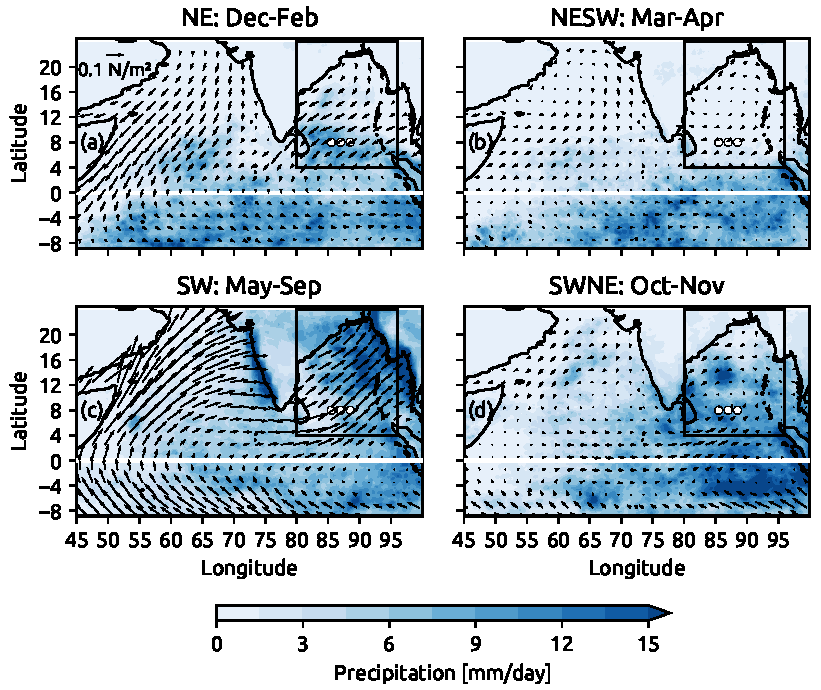
\includegraphics[width=33pc]{figure1-ppt.pdf}
\caption{\label{fig:ppt}
Seasonal mean wind stress over the ocean from Tropflux \citep{Kumar2012} and precipitation from the TRMM Multi-satellite Precipitation Analysis dataset \citep{trmm} over the Indian Ocean basin north of 10\(\degree\)S averaged between December, 2013 and November, 2014. Black box marks Bay of Bengal bounds shown in Figure \ref{fig:spatial}. White dots mark mooring locations.}
\end{figure*}

\begin{figure*}
\centering
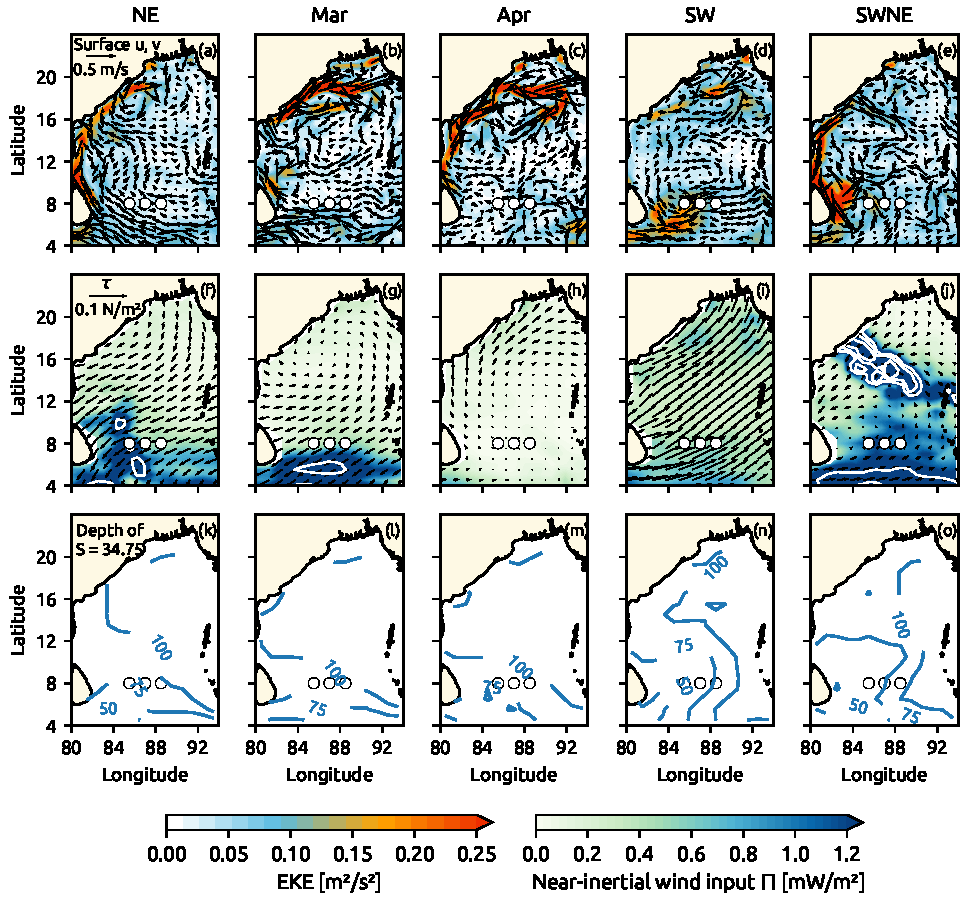
\includegraphics[width=\textwidth]{figure2-spatial-maps.pdf}
\caption{\label{fig:spatial}
Seasonal cycle of forcing and circulation in the Bay of Bengal for 2014. White dots mark mooring locations used in the study. (top) Seasonal mean geostrophic eddy kinetic energy (EKE) from altimeter sea surface height (SSH) in color; vectors indicate surface currents from seasonally averaged 5-day OSCAR estimate \citep{oscar,Bonjean2002}. (middle) Seasonal near-inertial energy input calculated using a slab ocean mixed layer model \(\Pi\slab\) (Appendix A). White contours are \(\Pi=\) \SIlist{2; 4; 10}{\milli\W\per\square\metre}. (bottom) 50, 75 and 100m depth contours of the 34.75 isohaline surface from the Argo mapped climatology of subsurface temperature and salinity \citep{Roemmich2009}. Similar results were obtained using the North Indian Ocean Atlas of \cite{Chatterjee2012}. The months of March and April are separated to emphasize the basin-wide weak mean wind stress and weak near-inertial input.}
\end{figure*}

\begin{figure*}
\centering
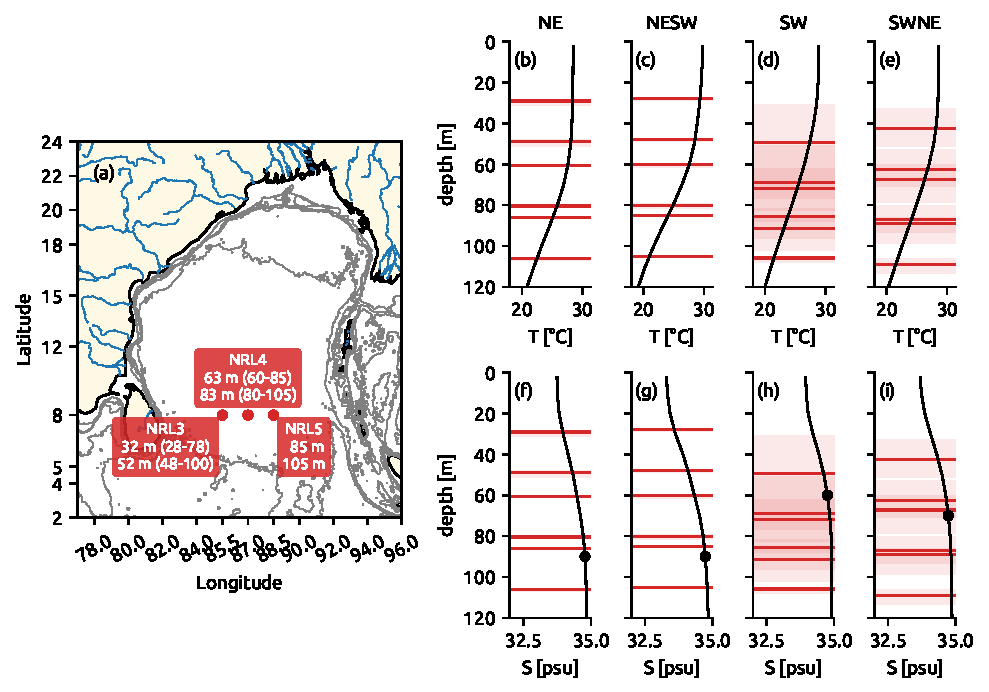
\includegraphics[width=\textwidth]{figure3-map.pdf}
\caption{\label{fig:map}
2014 \(\chi\)pod deployment at 8\(\degree\)N. (a) Locations of moorings. (b--i) Seasonal mean temperature (b--e) and salinity (f--i) profiles from the Argo climatology, averaged between 85.5\(\degree\)E and 88.5\(\degree\)E. These moorings experienced significant blowdown during the SW monsoon and the postmonsoon SWNE period. Horizontal lines and shading mark median and interquartile range of each \(\chi\)pod's depth for these two seasons. The black dot marks \(S=34.75\) psu. Temperature and salinity axes (lower and upper x-axes) are scaled such that axis limits represent equal jumps in density; panels (b--i) indicate that the mean stratification at the χpod depth levels is dominated by temperature in the long-term mean.}
\end{figure*}

\begin{figure*}
\centering
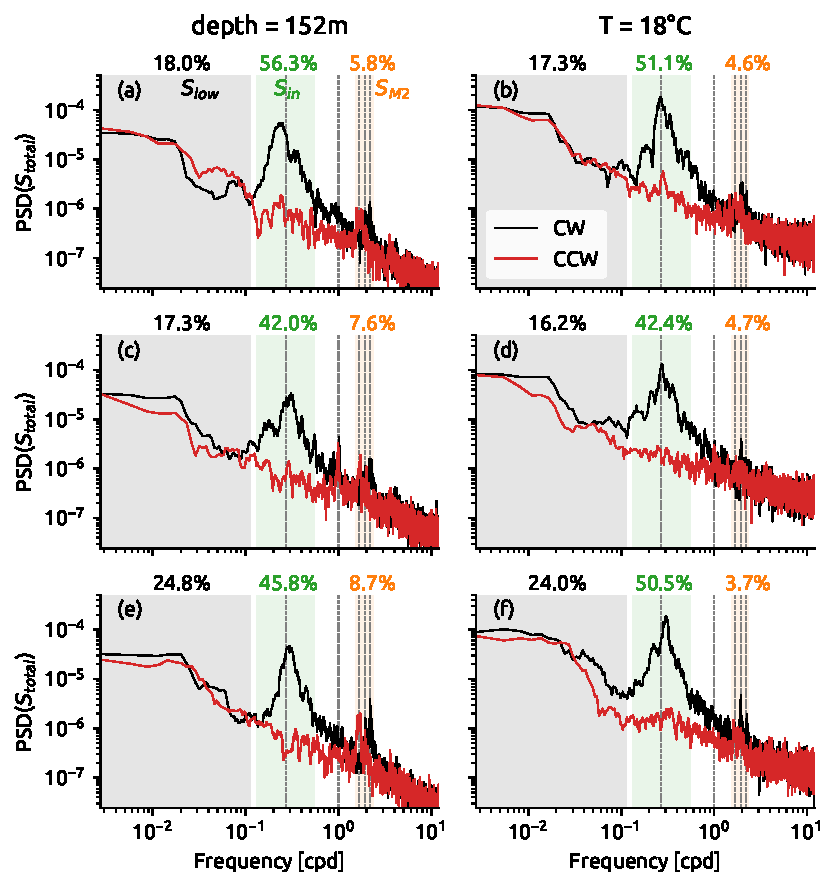
\includegraphics[width=39pc]{figure4-nrl-spectra.pdf}
\caption{\label{fig:nrlspectra}
Rotary power spectral density of total shear \(S\tot\) at all three moorings estimated using the multitaper method. (a, c, e) Eulerian estimate at \SI{152}{m}; (b, d, f) isothermal estimate at the \SI{18}{\celsius} isotherm. Lowpass, near-inertial and near-tidal bands (colored shading) as well as percentage of total shear variance in each band (colored text) are shown. Vertical lines mark \(f_0\), the diurnal frequency, \(ω_{M2} - f_0\) and \(ω_{M2} + f_0\). Clockwise and counter-clockwise spectra are in black and red respectively.}
\end{figure*}

\begin{figure*}
\centering
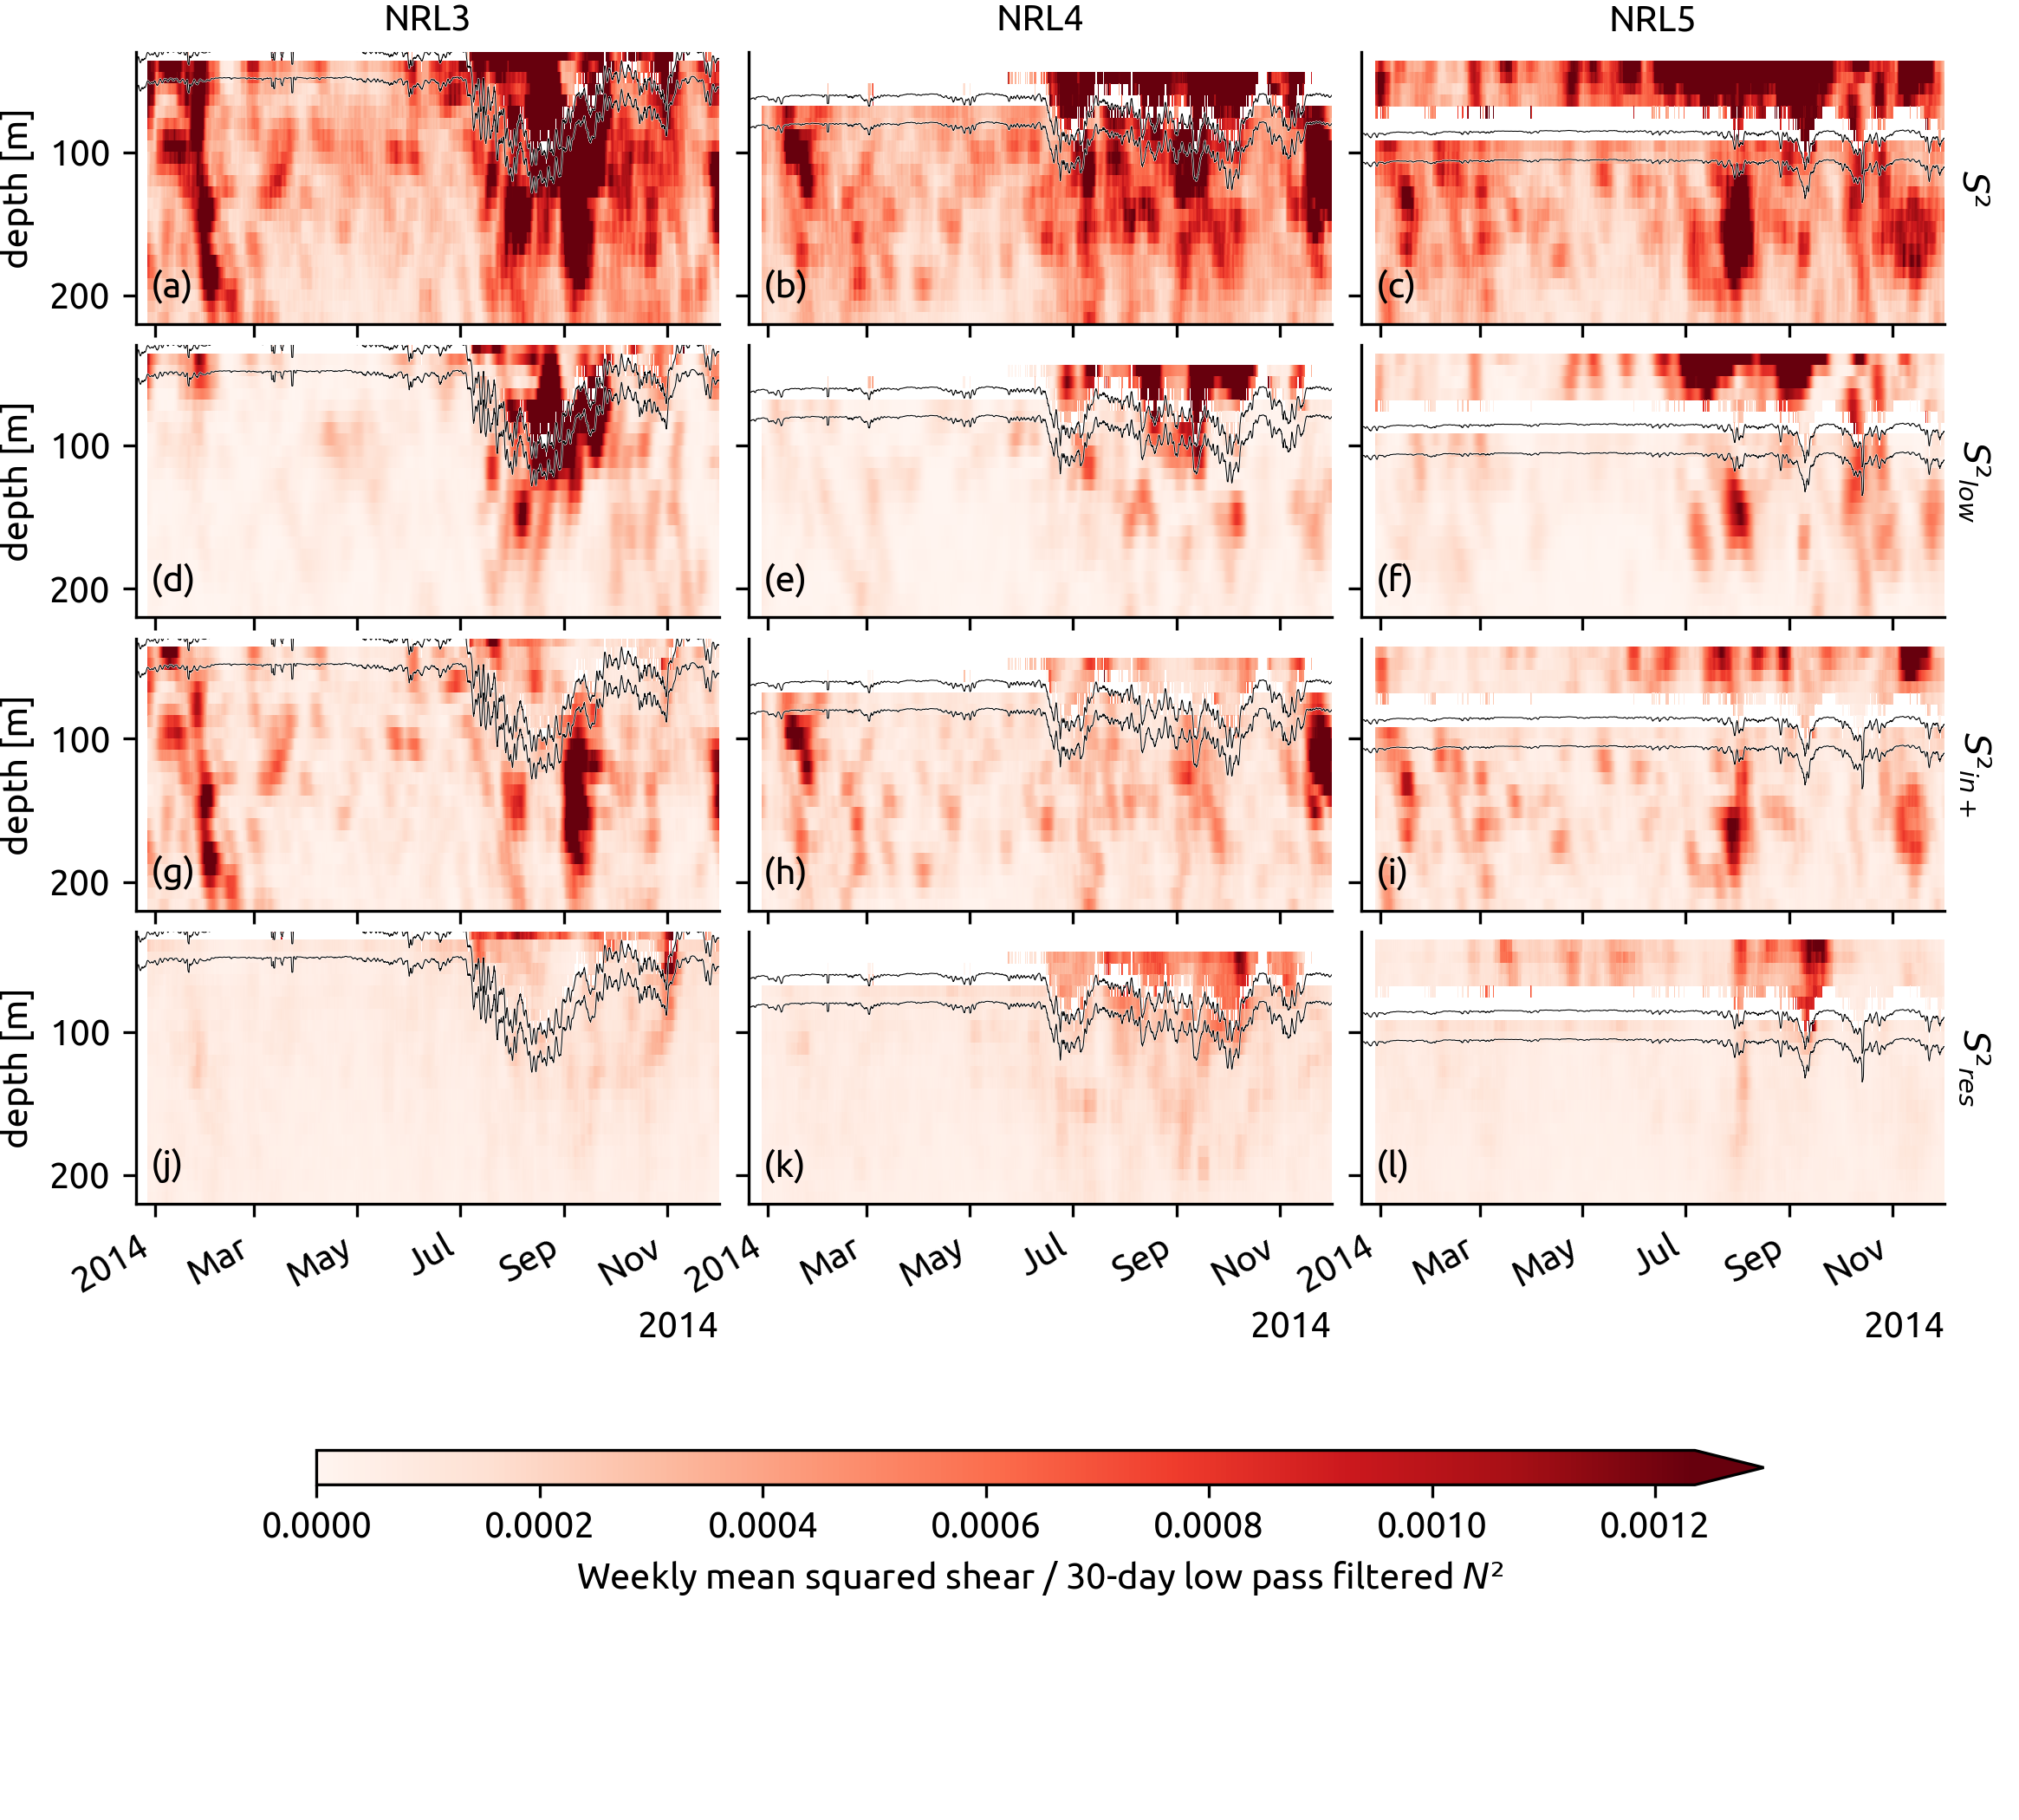
\includegraphics[width=\textwidth]{figure5-shears.png}
\caption{\label{fig:shears}
Weekly running mean-squared shear for the three moorings (top to bottom): (a-c) total shear \(S\tot^2\); (d-f) low-frequency shear \(S\low^2\); (g-i) total near-inertial shear \(S\niwp^2\) (j-l) residual shear \(S\res^2\). All components are normalized by the normalized by 30-day lowpass filtered \(N^2_T\). χpod depths for both χpods are shown in black in all panels. White contours mark levels \num{2e-3}, \num{4e-3} and \num{6e-3}.}
\end{figure*}

\begin{figure*}
\centering
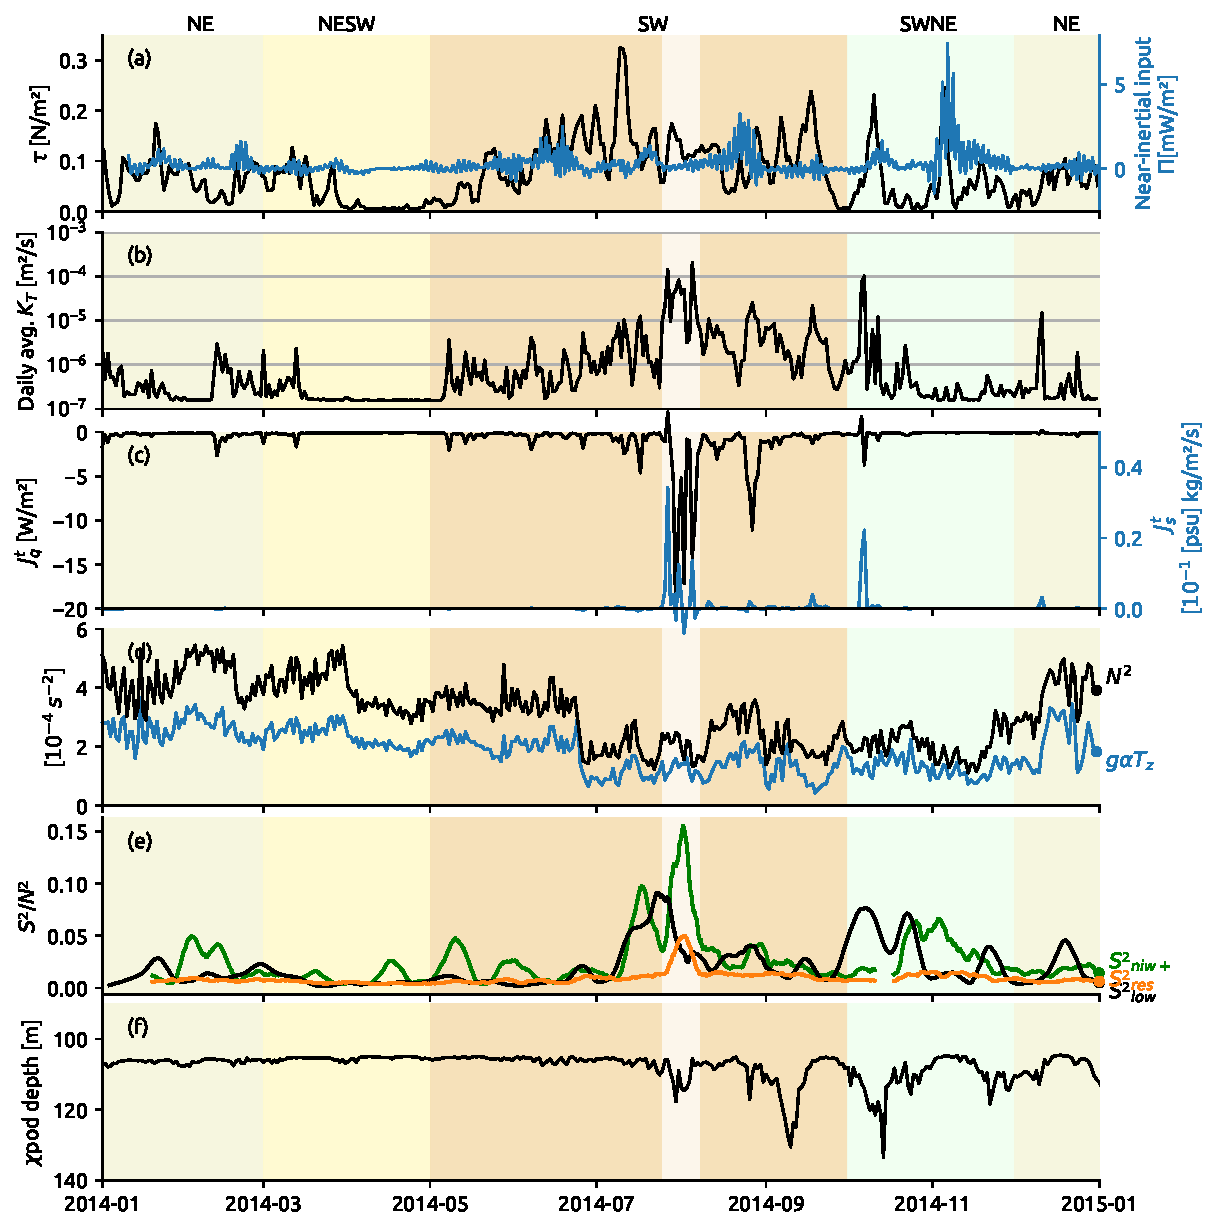
\includegraphics[width=\textwidth]{figure6-nrl5.pdf}
\caption{\label{fig:nrl}
A year of observations at NRL5, 105m. Time series of daily averaged quantities: (a) Tropflux wind stress; (b) daily averaged \(K_T\); (c) turbulent heat and salt fluxes \(J_q^t, J_s^t\); (d) Buoyancy frequency \(N^2\) and temperature contribution to \(N^2\), \(g \alpha T_z\); (e) Weekly running mean of filtered squared shear magnitude normalized by $N²$: low pass in black $S\low$, near-inertial bandpass $S\niwp$ in green and the residual $S\res$ in orange; (f) \(\chi\)pod depth. Background colors mark seasons; white region indicates time period shown in Figure \ref{fig:nrl5-niw}.}
\end{figure*}

\begin{figure*}
\centering
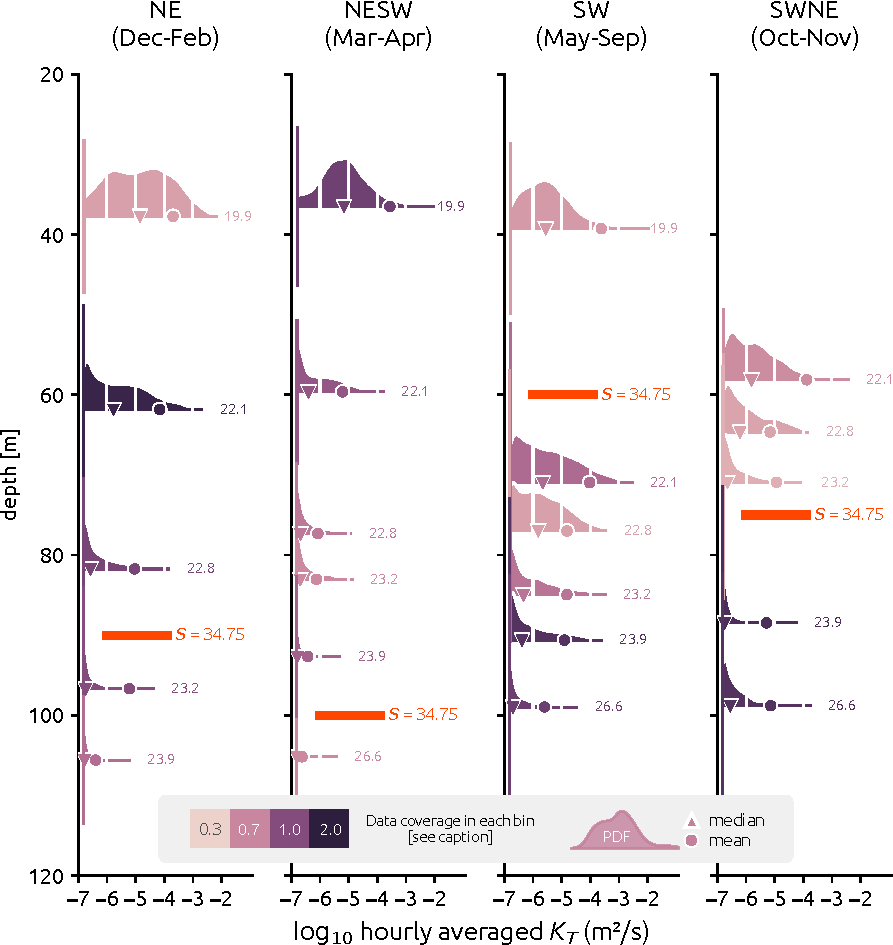
\includegraphics[width=\textwidth]{figure7-profile.pdf}
\caption{\label{fig:vert}
\small The seasonal cycle of \(K_T\) at 8°N. Vertical profile of hourly averaged \(K_T\) formed by combining all estimates in density bins (Section \ref{sec:profile}). PDFs as well as means and medians are shown. Bins are marked by \(\rho-1000\). Orange horizontal lines mark the climatological depth of the \(S=34.75\) isohaline at 8\(\degree\)N estimated using the Argo climatology. Vertical lines mark the standard deviation of measurement depths in each bin --- these lines tend to overlap each other. Each PDF is colored according to data coverage: one means that there is at least one hourly estimate for every hour in the season.}
\end{figure*}

\begin{figure}[htbp]
\centering
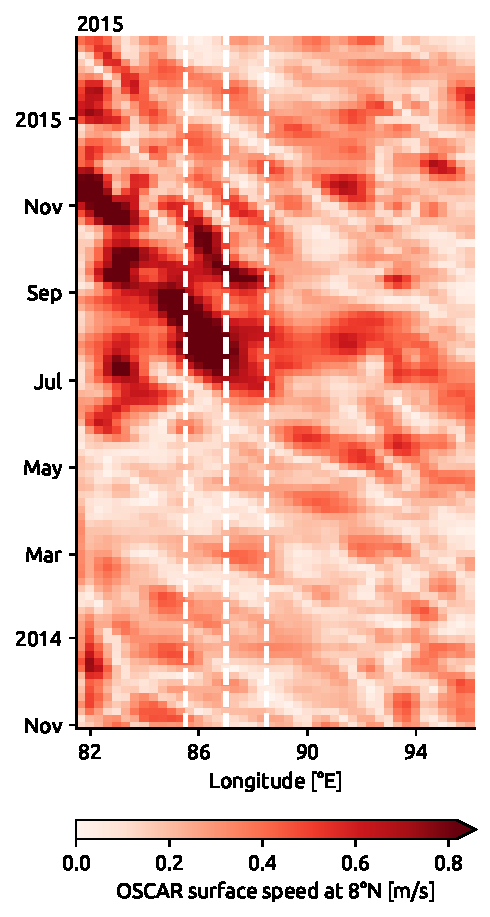
\includegraphics[height=0.5\textheight]{figure8-oscar.pdf}
\caption{\label{fig:hov}
Hovmoeller diagram of near-surface speed at 8°N as estimated in the OSCAR product. Vertical white dashed lines indicate mooring locations.}
\end{figure}

\begin{figure*}
\centering
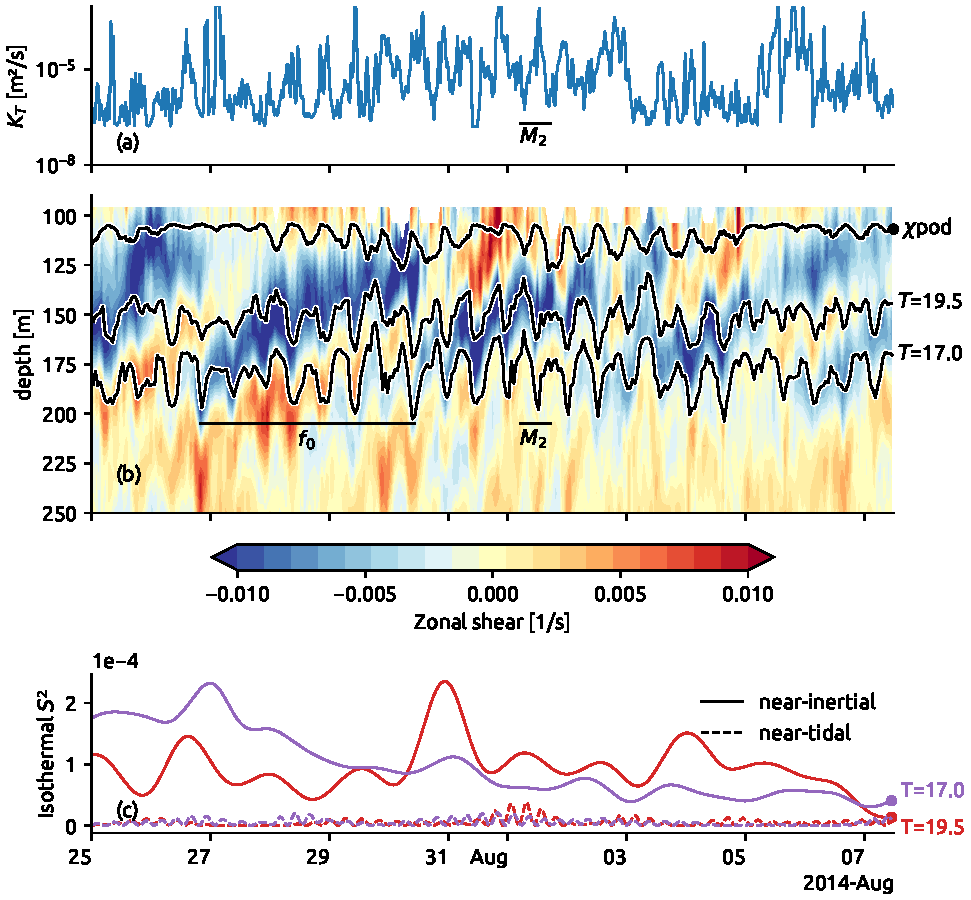
\includegraphics[width=\textwidth]{figure9-tidal-pumping.pdf}
\caption{\label{fig:nrl5-niw}
An example of pumping of the near-inertial shear layers past the \(\chi\)pod by the \(M_2\) tide at NRL5. The time period of focus is highlighted in white in Figure \ref{fig:nrl}. Time series of (a) turbulent diffusivity \(K_T\), (b) zonal shear and (c) near-inertial and near-tidal shear on two isotherms for a period of high mixing associated with downward propagating near-inertial energy. Horizontal lines indicate the inertial period (3.79 days; labelled \(f_0\)) and the \(M_2\) period (12.42 hours; labelled \(M_2\)). Also shown in (b) are the depth of the \(\chi\)pod and two isotherms (\SI{17}{\celsius}, \SI{19.5}{\celsius}). (c) Near-inertial shear dominates near-tidal shear by an order of magnitude on the two isotherms (\SI{17.0}{\celsius}, \SI{19.5}{\celsius}). The two time series are obtained by first interpolating total shear to isothermal space and then filtering as in Section \ref{sec:results}.}
\end{figure*}

\begin{figure*}
\centering
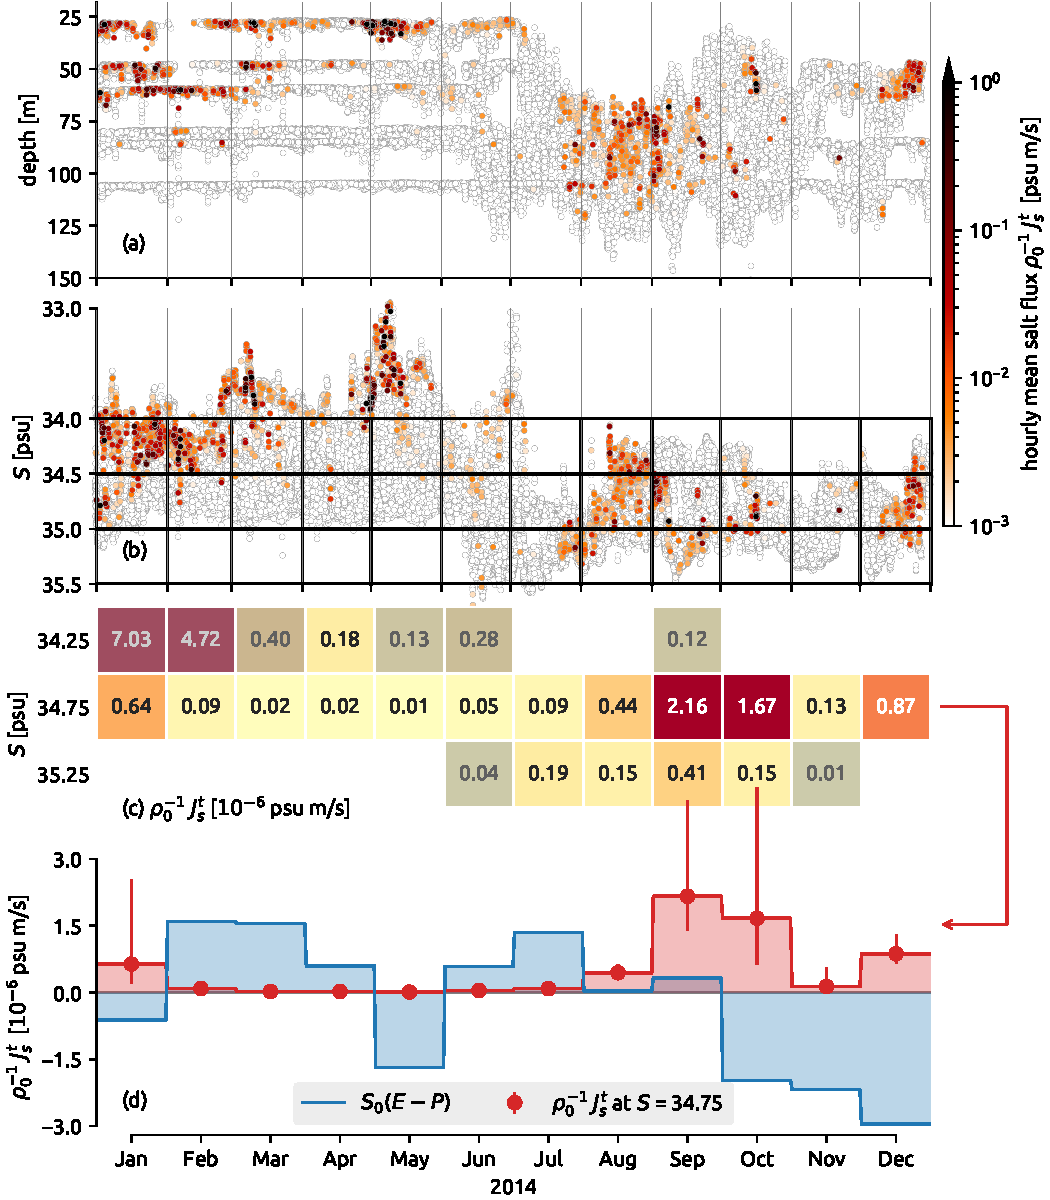
\includegraphics[width=\textwidth]{figure10-8n.pdf}
\caption{\label{fig:8njs}
Turbulent salt flux \(J_s^t\) at 8N. (a, b) Scatter plots of hourly averaged \(J_s^t\) in depth and salinity spaces respectively. Points with larger \(J_s^t\) are plotted over points with lower \(J_q^t\) so that high flux events are prominent. (c) Monthly averaged turbulent \(J_s^t\) through salinity surfaces \(S=34.25, 34.75\) and \(35.5\). These are estimated by bin averaging the values in (b) in bins with edges [34, 34.5, 35, 36]. Bins with less than one instrument-month of data are not shown. Those with less than two instrument months of data are grayed out. (d) Monthly averaged surface salinity flux \(S_0 (E-P)\) estimated using evaporation from OAFlux and precipitation from TRMM. \(S_0\) is assumed to be 32. In orange is \(J_s^t\) through \(S=34.75\) from (c) with bootstrap error bars.}
\end{figure*}
\end{document}